%! Author = Profesor
%! Date = 05/06/2024


\section{Ejercicios}\label{sec:ejercicios-UD3}

\subsection{Ejercicios Generales}\label{subsec:ejercicios-generales-UD3}

\begin{exercise}
    Representa las estructuras de Lewis de los compuestos
    \ch{HClO}, \ch{HClO2}, \ch{HClO3} y \ch{HClO4} (ten presente que el átomo
    de H está unido a un átomo de O).
    \begin{solu}
%        \begin{figure}[H]
%            \centering
%            \includegraphics[scale=.5]{images/imagesUD3EnlaceQuimico/UD3_Problemas/cuestiongeneral01}\label{fig:cuestiongeneral01}
%        \end{figure}
        En los cuatro oxoácidos el H está unido a un O (no directamente al Cl), y el Cl es el átomo central unido al resto de átomos de O.

        \textbf{\ch{HClO}}: \(\ch{H-O-Cl}\). El O tiene dos pares solitarios y el Cl tiene tres pares solitarios. Todos los átomos cumplen el octeto.

        \textbf{\ch{HClO2}}: \(\ch{H-O-Cl=O}\). El Cl forma un enlace sencillo con el O del \ch{OH} y un enlace doble con el otro O; le queda un par solitario al Cl. El O del \ch{OH} tiene dos pares solitarios y el O doblemente enlazado tiene dos pares solitarios.

        \textbf{\ch{HClO3}}: \(\ch{H-O-Cl(=O)2}\). El Cl forma un enlace sencillo con el O del \ch{OH} y dos enlaces dobles con los otros dos átomos de O; el Cl no tiene pares solitarios (expande su octeto).

        \textbf{\ch{HClO4}}: \(\ch{H-O-Cl(=O)3}\). El Cl forma un enlace sencillo con el O del \ch{OH} y tres enlaces dobles con los otros tres átomos de O; el Cl no tiene pares solitarios (expande su octeto al máximo).

        En los cuatro casos el Cl expande su capa de valencia por encima de ocho electrones (salvo en el \ch{HClO}), lo cual es posible porque el Cl dispone de orbitales \(d\) de valencia accesibles.
    \end{solu}
\end{exercise}

\begin{exercise}
    Representa las estructuras de Lewis de los iones \ch{ClO-},
    \ch{ClO2-}, \ch{ClO3-}, \ch{ClO4-}(ten presentes las estructuras de los
    oxoácidos que hiciste en el ejercicio anterior).
    \begin{solu}

%        \begin{figure}[H]
%            \centering
%            \includegraphics[scale=.5]{images/imagesUD3EnlaceQuimico/UD3_Problemas/cuestiongeneral02}
%        \end{figure}

        Estos iones se obtienen quitando el H de los oxoácidos del ejercicio anterior; el par de electrones del enlace \ch{O-H} queda íntegramente sobre el O, que adquiere la carga negativa.

        \textbf{\ch{ClO-}}: \([\ch{Cl-O}]^-\). El O tiene tres pares solitarios y carga \(-1\); el Cl tiene tres pares solitarios.

        \textbf{\ch{ClO2-}}: \([\ch{O-Cl=O}]^-\). Existen dos estructuras resonantes equivalentes en las que el enlace doble y la carga negativa se intercambian entre los dos átomos de O; en la estructura real la carga \(-1\) está deslocalizada por igual entre ambos O.

        \textbf{\ch{ClO3-}}: \([\ch{O-Cl(=O)2}]^-\). Hay tres estructuras resonantes; la carga negativa se reparte por igual entre los tres átomos de O.

        \textbf{\ch{ClO4-}}: \([\ch{Cl(=O)4}]^-\). Estructura tetraédrica con resonancia entre los cuatro átomos de O; la carga \(-1\) se distribuye equitativamente entre los cuatro O, lo que explica la gran estabilidad del ion perclorato.
    \end{solu}
\end{exercise}

\begin{exercise}
    Determina la entalpía de sublimación del cinc a partir de
    los siguientes datos, dados según el convenio de signos
    general de energías:
    \begin{figure}[H]
        \centering
        % [FIGURA ORIGINAL] \includegraphics[scale=.5]{images/imagesUD3EnlaceQuimico/UD3_Problemas/energiasejercicio12.png}
        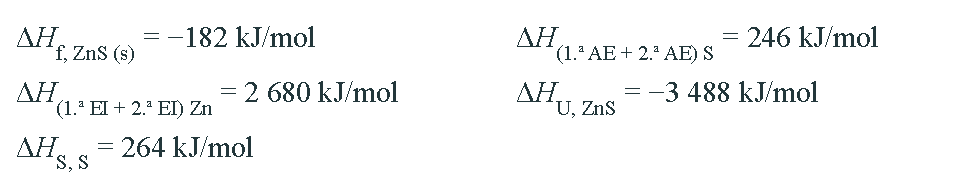
\includegraphics[width=0.7\linewidth]{FigurasSVG/UD3_Enlace_Quimico/pdf/UD3_E01_datos_ZnS.pdf}
    \end{figure}
    \begin{solu}

%        \begin{figure}[H]
%            \centering
%            \includegraphics[scale=.5]{images/imagesUD3EnlaceQuimico/UD3_Problemas/ejerciciogeneral03.png}
%        \end{figure}
%
        Los datos, según el convenio de signos general de energías, son:
        \(\entalpia{f, \ch{ZnS(s)}} = \energia[kj]{-182}\), \(\entalpia{S, S} = \energia[kj]{264}\), \(\entalpia{(1.ª EI + 2.ª EI), Zn} = \energia[kj]{2680}\), \(\entalpia{(1.ª AE + 2.ª AE), S} = \energia[kj]{246}\), \(U_{r, \ch{ZnS}} = \energia[kj]{-3488}\).

        El ciclo de Born-Haber para la formación de \ch{ZnS(s)} a partir de \ch{Zn(s)} y \ch{S(s)} es:
        \[
            \entalpia{f} = \entalpia{sub, Zn} + \entalpia{S, S} + \entalpia{(1.ª EI + 2.ª EI), Zn} + \entalpia{(1.ª AE + 2.ª AE), S} + U_r
        \]

        Despejando la entalpía de sublimación del cinc:
        \[
            \entalpia{sub, Zn} = \entalpia{f} - \entalpia{S, S} - \entalpia{(1.ª EI + 2.ª EI), Zn} - \entalpia{(1.ª AE + 2.ª AE), S} - U_r
        \]
        \[
            \entalpia{sub, Zn} = -182 - 264 - 2680 - 246 - (-3488) = \energia[kj]{116}
        \]

        La entalpía de sublimación del cinc es, por tanto, de \(\energia[kj]{116}\).
    \end{solu}
\end{exercise}


\begin{exercise}
    Asigna los valores de la energía de red correspondientes
    a los siguientes compuestos: \ch{AlCl3}, \ch{KCl}, \ch{CaCl2}, \ch{SrO},
    \ch{CsCl} y \ch{MgO}. Justifica tu respuesta.
    5 376 kJ/mol; 3 796 kJ/mol; 3 217 kJ/mol; 2 268 kJ/mol;
    701 kJ/mol; 657 kJ/mol.

    \begin{solu}

%        \begin{figure}[H]
%            \centering
%            \includegraphics[scale=.5]{images/imagesUD3EnlaceQuimico/UD3_Problemas/ejerciciogeneral04a.png}
%        \end{figure}

        La energía reticular (energía de red) es tanto mayor cuanto mayor es el producto de las cargas de los iones y cuanto menor es la distancia entre ellos (suma de sus radios iónicos), de acuerdo con la ley de Coulomb.

        \begin{itemize}
            \item \ch{AlCl3}: aunque el \ch{Al^{3+}} es pequeño, su carga (\(+3\)) es la más alta de todo el grupo, lo que domina el producto de cargas y le confiere la mayor energía reticular: \(\energia[kjmol]{5376}\).
            \item \ch{MgO} y \ch{SrO}: ambos con producto de cargas \(2\times2=4\), superior al de los cloruros univalentes. Como \ch{Mg^{2+}} es más pequeño que \ch{Sr^{2+}}, \ch{MgO} tiene mayor energía reticular: \(\energia[kjmol]{3796}\), frente a \(\energia[kjmol]{3217}\) del \ch{SrO}.
            \item \ch{CaCl2}: producto de cargas \(2\times1=2\), menor que en los óxidos anteriores: \(\energia[kjmol]{2268}\).
            \item \ch{KCl} y \ch{CsCl}: ambos con producto de cargas \(1\times1=1\), los menores del grupo. Como \ch{K+} es más pequeño que \ch{Cs+}, \ch{KCl} tiene mayor energía reticular: \(\energia[kjmol]{701}\), frente a \(\energia[kjmol]{657}\) del \ch{CsCl}.
        \end{itemize}
    \end{solu}
\end{exercise}


\begin{exercise}
    Ordena los compuestos \ch{AlCl3}, \ch{KCl}, \ch{CaCl2}, \ch{SrO}, \ch{CsCl} y \ch{MgO} según su solubilidad en agua.
    \begin{solu}
        La solubilidad depende de la energía de red. Serán más solubles
        los compuestos de menor energía de red, ya que es más probable
        que la energía de solvatación, debida a las interacciones de
        las moléculas del disolvente con los iones de la red, la compense:

        CsCl \textgreater KCl \textgreater \ch{CaCl2} \textgreater SrO \textgreater MgO \textgreater \ch{AlCl3}
    \end{solu}
\end{exercise}


\begin{exercise}
    Según la TRPECV, indica la geometría y la polaridad de
    estas moléculas (precisa la dirección y el sentido del momento
    dipolar de los enlaces y de las moléculas): \ch{PF3},
    \ch{H2S}, \ch{NH2OH}, \ch{CCl4}, \ch{CClH3}, \ch{BH3}, \ch{PF5}, \ch{OF2} y \ch{BeF2}.

    \begin{solu}

        Primero se hace la representación de Lewis de las moléculas
        y se determina la geometría de la molécula analizando los
        pares de electrones enlazantes y no enlazantes que rodean al
        átomo central. Después se analiza la polaridad de los enlaces
        que forma el átomo central con los otros átomos. Finalmente,
        se determina la polaridad de la molécula, teniendo en cuenta
        que \(\vec{\mu}_{\text{molécula}} = \sum \vec{\mu}_{\text{enlace}} \)

%        \begin{figure}[H]
%            \centering
%            \includegraphics[scale=.5]{images/imagesUD3EnlaceQuimico/UD3_Problemas/ejerciciogeneral06a.png}
%        \end{figure}
%
%        \begin{figure}[H]
%            \centering
%            \includegraphics[scale=.5]{images/imagesUD3EnlaceQuimico/UD3_Problemas/ejerciciogeneral06c.png}
%        \end{figure}
%
%        \begin{figure}[H]
%            \centering
%            \includegraphics[scale=.5]{images/imagesUD3EnlaceQuimico/UD3_Problemas/ejerciciogeneral06c.png}
%        \end{figure}
%
%        \begin{figure}[H]
%            \centering
%            \includegraphics[scale=.5]{images/imagesUD3EnlaceQuimico/UD3_Problemas/ejerciciogeneral06d.png}
%        \end{figure}
%        \begin{figure}[H]
%            \centering
%            \includegraphics[scale=.5]{images/imagesUD3EnlaceQuimico/UD3_Problemas/ejerciciogeneral06e.png}
%        \end{figure}

        % Los momentos dipolares de enlace se dibujan como flechas dirigidas hacia el átomo más electronegativo.
        \begin{center}
            % --- tabla antigua ---
            % \begin{tblr}{hlines, vlines, rows={abovesep=6pt, belowsep=6pt}, colspec={Q[l,m,wd=3.6cm] Q[c,m,wd=4.6cm] Q[c,m,wd=4.6cm]}, row{1}={bg=mybluecolour!15, font=\bfseries}, column{1}={font=\bfseries}}
                                                 % & \ch{PF3} & \ch{H2S} \\
                % Representación de Lewis          & \chemfig{\charge{90=\|,180=\|,270=\|}{F}-\charge{90=\:}{P}(-[6]\charge{0=\|,180=\|,270=\|}{F})-\charge{0=\|,90=\|,270=\|}{F}}
                                                 % & \chemfig{H-\charge{90=\:,270=\:}{S}-H} \\
                % Pares enlazantes                 & 3 & 2 \\
                % Pares no enlazantes              & 1 & 2 \\
                % Geometría del átomo central      & Tetraédrica & Tetraédrica \\
                % Geometría de la molécula         & Piramidal & Angular \\
                % \(EN\) de los elementos          & P (\num{2.1}); F (\num{4.0}) & S (\num{2.5}); H (\num{2.1}) \\
                % {Polaridad de la molécula \\ {\footnotesize\(\left(\vec{\mu}_{\text{molécula}} = \sum \vec{\mu}_{\text{enlace}}\right)\)}}
                                                 % & {\chemfig{\charge{90=\:}{P}(-[:-150,,,,-stealth]F)(-[:-30,,,,-stealth]F)-[:15,,,,-stealth]F} \\ \rule{0pt}{3.5ex}\(\vec{\mu}_{\text{molécula}} \neq 0\)}
                                                 % & {\chemfig{H-[:30,,,,-stealth]\charge{45=\:,135=\:}{S}-[:-30,,,,stealth-]H} \\ \rule{0pt}{3.5ex}\(\vec{\mu}_{\text{molécula}} \neq 0\)} \\
            % \end{tblr}
            % --- tabla nueva ---
            \begin{tabular}{@{}L{3.6cm} C{4.6cm} C{4.6cm}@{}}
                \toprule
                 & \textbf{\ch{PF3}} & \textbf{\ch{H2S}} \\
                \midrule
                \textbf{Representación de Lewis} & \chemfig{\charge{90=\|,180=\|,270=\|}{F}-\charge{90=\:}{P}(-[6]\charge{0=\|,180=\|,270=\|}{F})-\charge{0=\|,90=\|,270=\|}{F}} & \chemfig{H-\charge{90=\:,270=\:}{S}-H} \\[3pt]
                \textbf{Pares enlazantes} & 3 & 2 \\[3pt]
                \textbf{Pares no enlazantes} & 1 & 2 \\[3pt]
                \textbf{Geometría del átomo central} & Tetraédrica & Tetraédrica \\[3pt]
                \textbf{Geometría de la molécula} & Piramidal & Angular \\[3pt]
                \textbf{\(EN\) de los elementos} & P (\num{2.1}); F (\num{4.0}) & S (\num{2.5}); H (\num{2.1}) \\[3pt]
                \textbf{Polaridad de la molécula \newline {\footnotesize\(\left(\vec{\mu}_{\text{molécula}} = \sum \vec{\mu}_{\text{enlace}}\right)\)}} & \chemfig{\charge{90=\:}{P}(-[:-150,,,,-stealth]F)(-[:-30,,,,-stealth]F)-[:15,,,,-stealth]F} \newline \rule{0pt}{3.5ex}\(\vec{\mu}_{\text{molécula}} \neq 0\) & \chemfig{H-[:30,,,,-stealth]\charge{45=\:,135=\:}{S}-[:-30,,,,stealth-]H} \newline \rule{0pt}{3.5ex}\(\vec{\mu}_{\text{molécula}} \neq 0\) \\
                \bottomrule
            \end{tabular}
        \end{center}

        \begin{center}
            % --- tabla antigua ---
            % \begin{tblr}{hlines, vlines, rows={abovesep=6pt, belowsep=6pt}, colspec={Q[l,m,wd=3.6cm] Q[c,m,wd=4.6cm] Q[c,m,wd=4.6cm]}, row{1}={bg=mybluecolour!15, font=\bfseries}, column{1}={font=\bfseries}}
                                                 % & \ch{NH2OH} & \ch{CCl4} \\
                % Representación de Lewis          & \chemfig{H-\charge{90=\:}{N}(-[6]H)-\charge{90=\:,270=\:}{O}-H}
                                                 % & \chemfig{C(-[2]\charge{0=\|,90=\|,180=\|}{Cl})(-[4]\charge{90=\|,180=\|,270=\|}{Cl})(-[6]\charge{0=\|,180=\|,270=\|}{Cl})-\charge{0=\|,90=\|,270=\|}{Cl}} \\
                % Pares enlazantes                 & 3 & 4 \\
                % Pares no enlazantes              & 1 & 0 \\
                % Geometría del átomo central      & Tetraédrica & Tetraédrica \\
                % Geometría de la molécula         & Piramidal & Tetraédrica \\
                % \(EN\) de los elementos          & N (\num{3.0}); O (\num{3.5}); H (\num{2.1}) & C (\num{2.5}); Cl (\num{3.0}) \\
                % {Polaridad de la molécula \\ {\footnotesize\(\left(\vec{\mu}_{\text{molécula}} = \sum \vec{\mu}_{\text{enlace}}\right)\)}}
                                                 % & {\chemfig{\charge{90=\:}{N}(-[:-150,,,,stealth-]H)(-[:-30,,,,-stealth]OH)-[:15,,,,stealth-]H} \\ \rule{0pt}{3.5ex}\(\vec{\mu}_{\text{molécula}} \neq 0\)}
                                                 % & {\chemfig{C(-[2,,,,-stealth]Cl)(-[0,,,,-stealth]Cl)(-[:-130,,,,-stealth]Cl)-[:-50,,,,-stealth]Cl} \\ \rule{0pt}{3.5ex}\(\vec{\mu}_{\text{molécula}} = 0\)} \\
            % \end{tblr}
            % --- tabla nueva ---
            \begin{tabular}{@{}L{3.6cm} C{4.6cm} C{4.6cm}@{}}
                \toprule
                 & \textbf{\ch{NH2OH}} & \textbf{\ch{CCl4}} \\
                \midrule
                \textbf{Representación de Lewis} & \chemfig{H-\charge{90=\:}{N}(-[6]H)-\charge{90=\:,270=\:}{O}-H} & \chemfig{C(-[2]\charge{0=\|,90=\|,180=\|}{Cl})(-[4]\charge{90=\|,180=\|,270=\|}{Cl})(-[6]\charge{0=\|,180=\|,270=\|}{Cl})-\charge{0=\|,90=\|,270=\|}{Cl}} \\[3pt]
                \textbf{Pares enlazantes} & 3 & 4 \\[3pt]
                \textbf{Pares no enlazantes} & 1 & 0 \\[3pt]
                \textbf{Geometría del átomo central} & Tetraédrica & Tetraédrica \\[3pt]
                \textbf{Geometría de la molécula} & Piramidal & Tetraédrica \\[3pt]
                \textbf{\(EN\) de los elementos} & N (\num{3.0}); O (\num{3.5}); H (\num{2.1}) & C (\num{2.5}); Cl (\num{3.0}) \\[3pt]
                \textbf{Polaridad de la molécula \newline {\footnotesize\(\left(\vec{\mu}_{\text{molécula}} = \sum \vec{\mu}_{\text{enlace}}\right)\)}} & \chemfig{\charge{90=\:}{N}(-[:-150,,,,stealth-]H)(-[:-30,,,,-stealth]OH)-[:15,,,,stealth-]H} \newline \rule{0pt}{3.5ex}\(\vec{\mu}_{\text{molécula}} \neq 0\) & \chemfig{C(-[2,,,,-stealth]Cl)(-[0,,,,-stealth]Cl)(-[:-130,,,,-stealth]Cl)-[:-50,,,,-stealth]Cl} \newline \rule{0pt}{3.5ex}\(\vec{\mu}_{\text{molécula}} = 0\) \\
                \bottomrule
            \end{tabular}
        \end{center}

        \begin{center}
            % --- tabla antigua ---
            % \begin{tblr}{hlines, vlines, rows={abovesep=6pt, belowsep=6pt}, colspec={Q[l,m,wd=3.6cm] Q[c,m,wd=4.6cm] Q[c,m,wd=4.6cm]}, row{1}={bg=mybluecolour!15, font=\bfseries}, column{1}={font=\bfseries}}
                                                 % & \ch{CClH3} & \ch{BH3} \\
                % Representación de Lewis          & \chemfig{C(-[2]H)(-[4]H)(-[0]H)-[6]\charge{0=\|,180=\|,270=\|}{Cl}}
                                                 % & \chemfig{H-B(-[6]H)-H} \\
                % Pares enlazantes                 & 4 & 3 \\
                % Pares no enlazantes              & 0 & 0 \\
                % Geometría del átomo central      & Tetraédrica & Triangular \\
                % Geometría de la molécula         & Tetraédrica & Triangular \\
                % \(EN\) de los elementos          & C (\num{2.5}); H (\num{2.1}); Cl (\num{3.0}) & B (\num{2.0}); H (\num{2.1}) \\
                % {Polaridad de la molécula \\ {\footnotesize\(\left(\vec{\mu}_{\text{molécula}} = \sum \vec{\mu}_{\text{enlace}}\right)\)}}
                                                 % & {\chemfig{C(-[2,,,,-stealth]Cl)(-[0,,,,stealth-]H)(-[:-130,,,,stealth-]H)-[:-50,,,,stealth-]H} \\ \rule{0pt}{3.5ex}\(\vec{\mu}_{\text{molécula}} \neq 0\)}
                                                 % & {\chemfig{B(-[:150,,,,-stealth]H)(-[:30,,,,-stealth]H)-[6,,,,-stealth]H} \\ \rule{0pt}{3.5ex}\(\vec{\mu}_{\text{molécula}} = 0\)} \\
            % \end{tblr}
            % --- tabla nueva ---
            \begin{tabular}{@{}L{3.6cm} C{4.6cm} C{4.6cm}@{}}
                \toprule
                 & \textbf{\ch{CClH3}} & \textbf{\ch{BH3}} \\
                \midrule
                \textbf{Representación de Lewis} & \chemfig{C(-[2]H)(-[4]H)(-[0]H)-[6]\charge{0=\|,180=\|,270=\|}{Cl}} & \chemfig{H-B(-[6]H)-H} \\[3pt]
                \textbf{Pares enlazantes} & 4 & 3 \\[3pt]
                \textbf{Pares no enlazantes} & 0 & 0 \\[3pt]
                \textbf{Geometría del átomo central} & Tetraédrica & Triangular \\[3pt]
                \textbf{Geometría de la molécula} & Tetraédrica & Triangular \\[3pt]
                \textbf{\(EN\) de los elementos} & C (\num{2.5}); H (\num{2.1}); Cl (\num{3.0}) & B (\num{2.0}); H (\num{2.1}) \\[3pt]
                \textbf{Polaridad de la molécula \newline {\footnotesize\(\left(\vec{\mu}_{\text{molécula}} = \sum \vec{\mu}_{\text{enlace}}\right)\)}} & \chemfig{C(-[2,,,,-stealth]Cl)(-[0,,,,stealth-]H)(-[:-130,,,,stealth-]H)-[:-50,,,,stealth-]H} \newline \rule{0pt}{3.5ex}\(\vec{\mu}_{\text{molécula}} \neq 0\) & \chemfig{B(-[:150,,,,-stealth]H)(-[:30,,,,-stealth]H)-[6,,,,-stealth]H} \newline \rule{0pt}{3.5ex}\(\vec{\mu}_{\text{molécula}} = 0\) \\
                \bottomrule
            \end{tabular}
        \end{center}

        \begin{center}
            % --- tabla antigua ---
            % \begin{tblr}{hlines, vlines, rows={abovesep=6pt, belowsep=6pt}, colspec={Q[l,m,wd=3.6cm] Q[c,m,wd=4.6cm] Q[c,m,wd=4.6cm]}, row{1}={bg=mybluecolour!15, font=\bfseries}, column{1}={font=\bfseries}}
                                                 % & \ch{PF5} & \ch{OF2} \\
                % Representación de Lewis          & \chemfig{P(-[2]\charge{0=\|,90=\|,180=\|}{F})(-[:160]\charge{90=\|,180=\|,270=\|}{F})(-[:20]\charge{0=\|,90=\|,270=\|}{F})(-[:-120]\charge{0=\|,180=\|,270=\|}{F})-[:-60]\charge{0=\|,180=\|,270=\|}{F}}
                                                 % & \chemfig{\charge{90=\|,180=\|,270=\|}{F}-\charge{90=\:,270=\:}{O}-\charge{0=\|,90=\|,270=\|}{F}} \\
                % Pares enlazantes                 & 5 & 2 \\
                % Pares no enlazantes              & 0 & 2 \\
                % Geometría del átomo central      & Bipirámide triangular & Tetraédrica \\
                % Geometría de la molécula         & Bipirámide triangular & Angular \\
                % \(EN\) de los elementos          & P (\num{2.1}); F (\num{4.0}) & O (\num{3.5}); F (\num{4.0}) \\
                % {Polaridad de la molécula \\ {\footnotesize\(\left(\vec{\mu}_{\text{molécula}} = \sum \vec{\mu}_{\text{enlace}}\right)\)}}
                                                 % & {\chemfig{P(-[2,,,,-stealth]F)(-[6,,,,-stealth]F)(-[4,,,,-stealth]F)(-[:30,,,,-stealth]F)-[:-30,,,,-stealth]F} \\ \rule{0pt}{3.5ex}\(\vec{\mu}_{\text{molécula}} = 0\)}
                                                 % & {\chemfig{\charge{60=\:,120=\:}{O}(-[:-135,,,,-stealth]F)-[:-45,,,,-stealth]F} \\ \rule{0pt}{3.5ex}\(\vec{\mu}_{\text{molécula}} \neq 0\)} \\
            % \end{tblr}
            % --- tabla nueva ---
            \begin{tabular}{@{}L{3.6cm} C{4.6cm} C{4.6cm}@{}}
                \toprule
                 & \textbf{\ch{PF5}} & \textbf{\ch{OF2}} \\
                \midrule
                \textbf{Representación de Lewis} & \chemfig{P(-[2]\charge{0=\|,90=\|,180=\|}{F})(-[:160]\charge{90=\|,180=\|,270=\|}{F})(-[:20]\charge{0=\|,90=\|,270=\|}{F})(-[:-120]\charge{0=\|,180=\|,270=\|}{F})-[:-60]\charge{0=\|,180=\|,270=\|}{F}} & \chemfig{\charge{90=\|,180=\|,270=\|}{F}-\charge{90=\:,270=\:}{O}-\charge{0=\|,90=\|,270=\|}{F}} \\[3pt]
                \textbf{Pares enlazantes} & 5 & 2 \\[3pt]
                \textbf{Pares no enlazantes} & 0 & 2 \\[3pt]
                \textbf{Geometría del átomo central} & Bipirámide triangular & Tetraédrica \\[3pt]
                \textbf{Geometría de la molécula} & Bipirámide triangular & Angular \\[3pt]
                \textbf{\(EN\) de los elementos} & P (\num{2.1}); F (\num{4.0}) & O (\num{3.5}); F (\num{4.0}) \\[3pt]
                \textbf{Polaridad de la molécula \newline {\footnotesize\(\left(\vec{\mu}_{\text{molécula}} = \sum \vec{\mu}_{\text{enlace}}\right)\)}} & \chemfig{P(-[2,,,,-stealth]F)(-[6,,,,-stealth]F)(-[4,,,,-stealth]F)(-[:30,,,,-stealth]F)-[:-30,,,,-stealth]F} \newline \rule{0pt}{3.5ex}\(\vec{\mu}_{\text{molécula}} = 0\) & \chemfig{\charge{60=\:,120=\:}{O}(-[:-135,,,,-stealth]F)-[:-45,,,,-stealth]F} \newline \rule{0pt}{3.5ex}\(\vec{\mu}_{\text{molécula}} \neq 0\) \\
                \bottomrule
            \end{tabular}
        \end{center}

        \begin{center}
            % --- tabla antigua ---
            % \begin{tblr}{hlines, vlines, rows={abovesep=6pt, belowsep=6pt}, colspec={Q[l,m,wd=6cm] Q[c,m,wd=4.6cm]}, row{1}={bg=mybluecolour!15, font=\bfseries}, column{1}={font=\bfseries}}
                                                 % & \ch{BeF2} \\
                % Representación de Lewis          & \chemfig{\charge{90=\:,180=\:,270=\:}{F}-Be-\charge{0=\:,90=\:,270=\:}{F}} \\
                % Pares enlazantes                 & 2 \\
                % Pares no enlazantes              & 0 \\
                % Geometría del átomo central      & Lineal \\
                % Geometría de la molécula         & Lineal \\
                % \(EN\) de los elementos          & Be (\num{1.5}); F (\num{4.0}) \\
                % {Polaridad de la molécula \\ {\footnotesize\(\left(\vec{\mu}_{\text{molécula}} = \sum \vec{\mu}_{\text{enlace}}\right)\)}}
                                                 % & {\chemfig{F-[,,,,stealth-]Be-[,,,,-stealth]F} \\ \rule{0pt}{3.5ex}\(\vec{\mu}_{\text{molécula}} = 0\)} \\
            % \end{tblr}
            % --- tabla nueva ---
            \begin{tabular}{@{}L{6cm} C{4.6cm}@{}}
                \toprule
                 & \textbf{\ch{BeF2}} \\
                \midrule
                \textbf{Representación de Lewis} & \chemfig{\charge{90=\:,180=\:,270=\:}{F}-Be-\charge{0=\:,90=\:,270=\:}{F}} \\[3pt]
                \textbf{Pares enlazantes} & 2 \\[3pt]
                \textbf{Pares no enlazantes} & 0 \\[3pt]
                \textbf{Geometría del átomo central} & Lineal \\[3pt]
                \textbf{Geometría de la molécula} & Lineal \\[3pt]
                \textbf{\(EN\) de los elementos} & Be (\num{1.5}); F (\num{4.0}) \\[3pt]
                \textbf{Polaridad de la molécula \newline {\footnotesize\(\left(\vec{\mu}_{\text{molécula}} = \sum \vec{\mu}_{\text{enlace}}\right)\)}} & \chemfig{F-[,,,,stealth-]Be-[,,,,-stealth]F} \newline \rule{0pt}{3.5ex}\(\vec{\mu}_{\text{molécula}} = 0\) \\
                \bottomrule
            \end{tabular}
        \end{center}

    \end{solu}
\end{exercise}

\begin{exercise}
    Haz un estudio de la estructura de la molécula
    \chemfig{CH_2Cl-C~N}. Indica qué orbitales forman cada enlace y
    cómo son los ángulos de enlace.
    \begin{solu}
%        \begin{figure}[H]
%            \centering
%            \includegraphics[scale=.6]{images/imagesUD3EnlaceQuimico/UD3_Problemas/ejerciciogeneral07.png}
%        \end{figure}
        La molécula \(\ch{CH2Cl-C+N}\) (cloroacetonitrilo) tiene dos átomos de carbono con hibridaciones distintas:

        \begin{itemize}
            \item El carbono metilénico (\(\ch{CH2Cl}\)) presenta hibridación \(sp^3\): forma cuatro enlaces \(\sigma\) sencillos (dos con H, mediante solapamiento \(sp^3\)-\(s\); uno con Cl, mediante solapamiento \(sp^3\)-\(p\); y uno con el otro C, mediante solapamiento \(sp^3\)-\(sp\)). Los ángulos de enlace en torno a este carbono son de, aproximadamente, \(109{,}5°\) (geometría tetraédrica).
            \item El carbono nitrílico presenta hibridación \(sp\): forma un enlace \(\sigma\) sencillo con el carbono anterior (solapamiento \(sp\)-\(sp^3\)) y un enlace triple con el N, constituido por un enlace \(\sigma\) (solapamiento \(sp\)-\(sp\)) y dos enlaces \(\pi\) (solapamiento de los dos orbitales \(p\) no hibridados de cada átomo, perpendiculares entre sí). El ángulo \(\ch{C-C+N}\) es de \(180°\) (geometría lineal en torno a este carbono).
            \item El átomo de N, también con hibridación \(sp\), completa el enlace triple con el carbono y aloja un par de electrones solitario en el orbital \(sp\) restante, dirigido en línea recta con el resto de la molécula.
        \end{itemize}
    \end{solu}
\end{exercise}


\begin{exercise}
    Para las moléculas \chemfig{H-CHO}, \ch{CH3OH} y \ch{CH3OCH3}:
    a) Deduce a partir de sus estructuras de Lewis cuál tiene
    menor longitud de enlace CO.
    b) Justifica si alguna de ellas presenta enlace de H.
    \begin{solu}
%        \begin{figure}[H]
%            \centering
%            \includegraphics[scale=.6]{images/imagesUD3EnlaceQuimico/UD3_Problemas/ejerciciogeneral08.png}
%        \end{figure}
        a) El \ch{H-CHO} (metanal) tiene un enlace \ch{C=O} doble, con longitud de enlace corta (mayor orden de enlace, dos pares de electrones compartidos), mientras que el \ch{CH3OH} y el \ch{CH3OCH3} tienen un enlace \ch{C-O} sencillo, más largo. Por tanto, el \ch{H-CHO} presenta \textbf{menor longitud de enlace \ch{C-O}} que los otros dos compuestos.

        b) El enlace de hidrógeno se establece entre un átomo de H unido a un átomo muy electronegativo (F, O, N) y un par solitario de otro átomo electronegativo de una molécula vecina; requiere, por tanto, un grupo \ch{O-H} (o \ch{N-H}, \ch{F-H}). Solo el \ch{CH3OH} posee un grupo \ch{-OH}, por lo que es la única de las tres moléculas capaz de establecer enlaces de H entre sus propias moléculas (actuando a la vez como dador y aceptor). El \ch{H-CHO} y el \ch{CH3OCH3} tienen átomo de O, por lo que pueden actuar como \emph{aceptores} de enlace de H frente a otras moléculas que sí tengan \ch{-OH} (como el agua), pero no pueden formar enlaces de H entre sus propias moléculas, al carecer de H unido a un átomo electronegativo.
    \end{solu}
\end{exercise}

\begin{exercise}
    Dadas las moléculas \ch{H2O}, \ch{HF}, \ch{H2}, \ch{CH4} y \ch{NH3}, contesta
    justificadamente a cada una de las siguientes cuestiones:
    a) ¿Cuál o cuáles son polares?
    b) ¿Cuál presenta el enlace con mayor contribución iónica?
    c) ¿Cuál presenta el enlace con mayor contribución covalente?
    d) ¿Cuál o cuáles pueden presentar enlace de hidrógeno?
    \begin{solu}
%        \begin{figure}[H]
%            \centering
%            \includegraphics[scale=.6]{images/imagesUD3EnlaceQuimico/UD3_Problemas/ejerciciogeneral08.png}
%        \end{figure}
        a) \ch{H2O}: molécula angular con enlaces polares → molécula polar;
        \ch{HF}: enlace polar, molécula polar; \ch{H2}: enlace apolar, molécula
        apolar; \ch{CH4}: enlaces poco polares, molécula tetraédrica
        perfectamente simétrica → molécula apolar; NH3: enlaces
        polares, molécula piramidal → molécula polar.
        b) El enlace con mayor contribución iónica es el enlace más
        polar: enlace \ch{H-F}.
        c) El enlace con mayor contribución covalente es el enlace
        menos polar: enlace \ch{H-H}.
        d) Pueden presentar enlaces de H las moléculas que contengan
        enlaces \ch{-OH}, \ch{F-H} y \ch{-NH}. En este caso, las moléculas
        de \ch{H2O}, \ch{HF} y \ch{NH3}.
    \end{solu}
\end{exercise}


\begin{exercise}
    Indica, razonadamente, qué tipo de interacción o enlace
    químico se rompe para:
    a) Fundir cloruro de potasio. c) Hervir agua.
    b) Disolver yodo en benceno. d) Sublimar sodio.
    \begin{solu}

%        \begin{figure}[H]
%            \centering
%            \includegraphics[scale=.6]{images/imagesUD3EnlaceQuimico/UD3_Problemas/ejerciciogeneral10a.png}
%            \includegraphics[scale=.6]{images/imagesUD3EnlaceQuimico/UD3_Problemas/ejerciciogeneral10b.png}
%        \end{figure}

        \begin{itemize}
            \item[a)] \textbf{Fundir cloruro de potasio}: se rompe el \textbf{enlace iónico}, es decir, la red cristalina que mantiene unidos los iones \ch{K+} y \ch{Cl-}.
            \item[b)] \textbf{Disolver yodo en benceno}: se rompen las \textbf{fuerzas de dispersión de London} (van der Waals) que mantienen unidas entre sí las moléculas apolares de \ch{I2}.
            \item[c)] \textbf{Hervir agua}: se rompen los \textbf{enlaces de hidrógeno} que mantienen unidas las moléculas de \ch{H2O} en estado líquido.
            \item[d)] \textbf{Sublimar sodio}: se rompe el \textbf{enlace metálico} que mantiene unidos los átomos de Na en la red metálica.
        \end{itemize}
    \end{solu}
\end{exercise}



\begin{exercise}
    A la presión atmosférica, el \ch{H2O} tiene un punto de ebullición
    de 100 °C; el \ch{CH3OH}, de 64,5 °C, y el \ch{C2H5OH}, de
    78 °C. Justifica este hecho sobre la base de los enlaces
    intermoleculares que se dan en esas sustancias.
    \begin{solu}
        Las tres sustancias presentan enlace de H, ya que tienen
        \ch{O-H}. Cada molécula de agua puede formar dos enlaces de
        H, ya que tiene dos grupos OH, mientras que una molécula
        de etanol o de metanol solo puede formar uno; por esta razón,
        el punto de ebullición del agua es mayor. Entre los dos
        alcoholes, el de mayor punto de ebullición es el etanol, ya
        que, tratándose de moléculas de la misma serie homóloga,
        la de mayor masa molar es la que presenta mayor punto de
        ebullición.
    \end{solu}
\end{exercise}


\begin{exercise}
    Calcula la energía de red (energía reticular) del cloruro de magnesio tomando como datos: $\entalpia{sub} =  \energia[kj]{147.7}$, $EI (\text{1º y 2º}) = \energia[kj]{2188}$,  $\entalpia{dis} =  \energia[kj]{244}$, $AE = \energia[kj]{-348}$, $\entalpia{f} =  \energia[kjmol]{-642}$
    \begin{solu}

        El ciclo de Born-Haber para la formación de \ch{MgCl2(s)} a partir de \ch{Mg(s)} y \ch{Cl2(g)} es:
        \[
            \entalpia{f} = \entalpia{sub} + EI(\text{1º y 2º}) + \entalpia{dis} + 2 \, AE + U_r
        \]

        El factor 2 en la afinidad electrónica se debe a que se forman dos iones \ch{Cl-} por cada unidad de \ch{MgCl2}, mientras que la disociación de \ch{Cl2} ya proporciona directamente los dos átomos de Cl necesarios.

        Despejando la energía reticular:
        \[
            U_r = \entalpia{f} - \entalpia{sub} - EI(\text{1º y 2º}) - \entalpia{dis} - 2 \, AE
        \]
        \[
            U_r = -642 - 147{,}7 - 2188 - 244 - 2\cdot(-348) = \energia[kj]{-2525,7}
        \]

        La energía de red del cloruro de magnesio es, por tanto, de \(\energia[kj]{-2525,7}\) (energía liberada al formarse el sólido iónico a partir de los iones gaseosos).
    \end{solu}
\end{exercise}

\begin{exercise}
    Calcula la afinidad electrónica del oxígeno para dar \ch{O\mch[2]} (suma de la primera y segunda AE), a partir del ciclo de Born-Haber del óxido de sodio. Datos: $\entalpia{f, \ch{Na2O (s)}} = \energia[kjmol]{-414,2} -414.2$, $\entalpia{dis,\ch{O2}} = \energia[kjmol]{494}$, $\entalpia{sub, \ch{Na}} = \energia[kjmol]{107,3}$, $EI_{Na} = \energia[kjmol]{495,8}$, $U_r{\ch{Na2O(s)}} = \energia[kjmol]{-2604,4}$
    \begin{solu}

%        \begin{figure}[H]
%            \centering
%            \includegraphics[scale=.5]{images/imagesUD3EnlaceQuimico/UD3_Problemas/ejerciciogeneral13.png}
%            %\caption{}
%            %\label{fig:}
%        \end{figure}

        El ciclo de Born-Haber para la formación de \ch{Na2O(s)} a partir de \ch{2Na(s)} y \(\frac{1}{2}\)\ch{O2(g)} es:
        \[
            \entalpia{f} = 2\,\entalpia{sub, Na} + 2\,EI_{Na} + \tfrac{1}{2}\entalpia{dis, \ch{O2}} + AE_{(1.ª+2.ª), O} + U_r
        \]

        Despejando la suma de la primera y segunda afinidad electrónica del oxígeno:
        \[
            AE_{(1.ª+2.ª), O} = \entalpia{f} - 2\,\entalpia{sub, Na} - 2\,EI_{Na} - \tfrac{1}{2}\entalpia{dis, \ch{O2}} - U_r
        \]
        \[
            AE_{(1.ª+2.ª), O} = -414{,}2 - 2\cdot107{,}3 - 2\cdot495{,}8 - \tfrac{1}{2}\cdot494 - (-2604{,}4) = \energia[kjmol]{737,0}
        \]

        La suma de la primera y segunda afinidad electrónica del oxígeno es de \(\energia[kjmol]{737,0}\), un valor positivo (proceso globalmente endotérmico), ya que la primera AE del O es exotérmica pero la segunda (incorporar un electrón a un ion \ch{O-} ya negativo) es muy endotérmica, y esta última domina la suma.
    \end{solu}
\end{exercise}



\begin{exercise}
    Asigna los puntos de fusión \temperatura[c]{642}, \temperatura[c]{734}, \temperatura[c]{996} aproximados a cada una de estas sustancias, \ch{KBr}, \ch{RbI} y \ch{NaF}.
    Justifícalo según los datos de la tabla.
    \begin{figure}[H]
        \centering
        \begin{tblr}{|c|c|c|c|}
            \hline
            Compuesto            & \ch{KBr} & \ch{RbI} & \ch{NaF } \\
            \hline
            Energía de reticular & 682      & 630      & 923       \\
            \hline
            Punto de fusión & 734 & 642 & 996 \\
            \hline
        \end{tblr}

    \end{figure}
%    \begin{figure}[H]
%        \centering
%        \includegraphics[scale=0.5]{images/imagesUD3EnlaceQuimico/UD3_Problemas/tabla_ejer_fusion.png}
%        %\caption{}
%        \label{fig:tabla_ejer}
%    \end{figure}
    \begin{solu}

        Para fundir un compuesto iónico, hay que romper la red cristalina. Por tanto, el punto de fusión es tanto más alto cuanto mayor sea la energía reticular (energía de red).

    \end{solu}
\end{exercise}


\begin{exercise}
    Explica qué le ocurre a la energía reticular de los compuestos iónicos del tipo \ch{A^{x+}} y \ch{B^{y-}} si:
    \begin{enumerate}[label=\letraminuscula]
        \item Se duplica la carga del anión.
        \item Se reduce a la mitad la carga del catión.
        \item Aumenta el tamaño del anión.
        \item Aumenta el tamaño del catión.
        \item Se incrementa el coeficiente o factor de Born.
        \item Los iones pasan de tener estructura de tipo Ar a tenerla tipo Ne.
        \item Disminuye la constante de Madelung.
    \end{enumerate}
    \begin{solu}

        La energía reticular sigue, de forma aproximada, la expresión de Born-Landé:
        \[
            U_r = -\frac{N_A \, M \, z_+ \, z_- \, e^2}{4\pi\varepsilon_0 \, r_0}\left(1-\frac{1}{n}\right)
        \]
        donde \(z_+\) y \(z_-\) son las cargas de los iones, \(r_0\) la distancia entre sus centros (suma de radios iónicos), \(M\) la constante de Madelung y \(n\) el factor (exponente) de Born.

        \begin{enumerate}[label=\letraminuscula]
            \item Al duplicarse la carga del anión, el producto \(z_+ z_-\) se duplica, por lo que la energía reticular \textbf{se duplica aproximadamente} (en valor absoluto aumenta).
            \item Al reducirse a la mitad la carga del catión, el producto \(z_+ z_-\) se reduce a la mitad, por lo que la energía reticular \textbf{se reduce aproximadamente a la mitad}.
            \item Al aumentar el tamaño del anión, aumenta \(r_0\), por lo que la energía reticular \textbf{disminuye} (en valor absoluto).
            \item Al aumentar el tamaño del catión, aumenta \(r_0\), por lo que la energía reticular \textbf{disminuye} (en valor absoluto), igual que en el caso anterior.
            \item Al incrementarse el factor de Born \(n\), el término \(\left(1-\dfrac{1}{n}\right)\) aumenta (se acerca a 1), por lo que la energía reticular \textbf{aumenta ligeramente} en valor absoluto.
            \item Los iones con estructura tipo Ar tienen un factor de Born mayor (\(n\approx9\)) que los de tipo Ne (\(n\approx7\)). Al pasar de tipo Ar a tipo Ne, \(n\) disminuye, el término \(\left(1-\dfrac{1}{n}\right)\) disminuye y, por tanto, la energía reticular \textbf{disminuye ligeramente} en valor absoluto.
            \item Como \(U_r\) es directamente proporcional a la constante de Madelung \(M\), si esta disminuye, la energía reticular \textbf{disminuye} en valor absoluto.
        \end{enumerate}
    \end{solu}
\end{exercise}

\begin{exercise}
    %!Página 112 Ejercicio 1
    \begin{enumerate}[label=\letraminuscula]
        \item ¿Qué es un enlace químico?
        \item ¿Qué tipos de enlace conoces?
        \item ¿Entre qué elementos de la tabla periódica se produce cada uno de los enlaces?
    \end{enumerate}
    Cita tres sustancias con cada uno de los tres tipos principales de enlace que conoces.
    \begin{solu}

        \begin{enumerate}[label=\letraminuscula]
            \item Un enlace químico es el conjunto de fuerzas que mantiene unidos a los átomos o iones cuando forman moléculas, cristales o redes metálicas.
            \item Los tres tipos principales de enlace son el \textbf{iónico}, el \textbf{covalente} y el \textbf{metálico}.
            \item El enlace \textbf{iónico} se produce entre un elemento metálico (grupos 1-2 y metales de transición, baja electronegatividad) y un elemento no metálico (grupos 16-17, alta electronegatividad), con una diferencia de electronegatividad grande. El enlace \textbf{covalente} se produce entre elementos no metálicos (parte derecha de la tabla), con electronegatividades altas y similares. El enlace \textbf{metálico} se produce entre átomos de elementos metálicos entre sí.
        \end{enumerate}

        Ejemplos: enlace iónico: \ch{NaCl}, \ch{CaO}, \ch{KBr}. Enlace covalente: \ch{H2O}, \ch{CO2}, \ch{HCl}. Enlace metálico: Fe, Cu, Na.
    \end{solu}
\end{exercise}

\begin{exercise}
    %!Página 112 Ejercicio 10 Bruño
    ¿Es cierta la siguiente afirmación: Solo los compuestos pueden tener enlace iónico?
    \begin{solu}

        Sí, es cierta. El enlace iónico se produce por transferencia de electrones entre átomos de electronegatividades muy distintas (un metal, que cede electrones, y un no metal, que los capta), formando un catión y un anión que se atraen electrostáticamente. Como esta transferencia solo tiene sentido entre átomos de \textbf{elementos diferentes}, el enlace iónico siempre da lugar a un \textbf{compuesto} (sustancia formada por al menos dos elementos distintos), y nunca a una sustancia elemental (formada por átomos de un único elemento, con igual electronegatividad, entre los que no puede haber transferencia neta de electrones).
    \end{solu}
\end{exercise}

\begin{exercise}
    %!Página 112 Ejercicio 11
    Escribe los iones que pueden formar los elementos: Li, Cs, Ag, Zn, Cu, Ti, F, O, As, N, I, Se, Te.
    \begin{solu}

        Los metales tienden a perder sus electrones de valencia para adquirir configuración de gas noble (o de capa \(d\) completa), formando cationes; los no metales tienden a ganar electrones hasta completar el octeto, formando aniones:

        \begin{itemize}
            \item Li \(\rightarrow\) \ch{Li+}
            \item Cs \(\rightarrow\) \ch{Cs+}
            \item Ag \(\rightarrow\) \ch{Ag+}
            \item Zn \(\rightarrow\) \ch{Zn^{2+}}
            \item Cu \(\rightarrow\) \ch{Cu+} y \ch{Cu^{2+}} (presenta dos estados de oxidación habituales)
            \item Ti \(\rightarrow\) \ch{Ti^{2+}}, \ch{Ti^{3+}} y \ch{Ti^{4+}} (siendo este último el más estable)
            \item F \(\rightarrow\) \ch{F-}
            \item O \(\rightarrow\) \ch{O^{2-}}
            \item As \(\rightarrow\) \ch{As^{3-}}
            \item N \(\rightarrow\) \ch{N^{3-}}
            \item I \(\rightarrow\) \ch{I-}
            \item Se \(\rightarrow\) \ch{Se^{2-}}
            \item Te \(\rightarrow\) \ch{Te^{2-}}
        \end{itemize}
    \end{solu}
\end{exercise}

\begin{exercise}
    %!Página 112 Ejercicio 12
    Escribe las estructuras de Lewis para los átomos neutros y para los iones del ejercicio anterior.
    \begin{solu}

        La estructura de Lewis de un átomo o ion se representa mediante su símbolo rodeado de puntos, uno por cada electrón de su capa de valencia:

        \begin{itemize}
            \item \textbf{Li} (1 e\(^-\) de valencia, \(2s^1\)) \(\rightarrow\) \textbf{Li\(^+\)}: pierde su único electrón de valencia y queda \textbf{sin electrones de valencia} (isoelectrónico con el He).
            \item \textbf{Cs} (1 e\(^-\) de valencia) \(\rightarrow\) \textbf{Cs\(^+\)}: pierde su electrón de valencia, sin electrones de valencia (isoelectrónico con el Xe).
            \item \textbf{Ag} (1 e\(^-\) de valencia, \(5s^1\)) \(\rightarrow\) \textbf{Ag\(^+\)}: pierde el electrón \(5s\), sin electrones de valencia \(s\)/\(p\) (queda con la subcapa \(4d^{10}\) completa).
            \item \textbf{Zn} (2 e\(^-\) de valencia, \(4s^2\)) \(\rightarrow\) \textbf{Zn\(^{2+}\)}: pierde los dos electrones \(4s\), sin electrones de valencia \(s\)/\(p\) (queda con la subcapa \(3d^{10}\) completa).
            \item \textbf{Cu} (1 e\(^-\) de valencia, \(4s^1\)) \(\rightarrow\) \textbf{Cu\(^+\)}: pierde el electrón \(4s\) (subcapa \(3d^{10}\) completa); \textbf{Cu\(^{2+}\)}: pierde además un electrón \(3d\) (subcapa \(3d^9\)).
            \item \textbf{Ti} (4 e\(^-\) de valencia, \(4s^23d^2\)) \(\rightarrow\) \textbf{Ti\(^{4+}\)}: pierde los cuatro electrones de valencia, sin electrones de valencia.
            \item \textbf{F} (7 e\(^-\) de valencia, tres pares y un electrón desapareado) \(\rightarrow\) \textbf{F\(^-\)}: gana un electrón y completa el octeto (cuatro pares de electrones).
            \item \textbf{O} (6 e\(^-\) de valencia, dos pares y dos electrones desapareados) \(\rightarrow\) \textbf{O\(^{2-}\)}: gana dos electrones y completa el octeto (cuatro pares).
            \item \textbf{As} (5 e\(^-\) de valencia) \(\rightarrow\) \textbf{As\(^{3-}\)}: gana tres electrones y completa el octeto (cuatro pares).
            \item \textbf{N} (5 e\(^-\) de valencia) \(\rightarrow\) \textbf{N\(^{3-}\)}: gana tres electrones y completa el octeto (cuatro pares).
            \item \textbf{I} (7 e\(^-\) de valencia) \(\rightarrow\) \textbf{I\(^-\)}: gana un electrón y completa el octeto (cuatro pares).
            \item \textbf{Se} (6 e\(^-\) de valencia) \(\rightarrow\) \textbf{Se\(^{2-}\)}: gana dos electrones y completa el octeto (cuatro pares).
            \item \textbf{Te} (6 e\(^-\) de valencia) \(\rightarrow\) \textbf{Te\(^{2-}\)}: gana dos electrones y completa el octeto (cuatro pares).
        \end{itemize}

        En todos los casos, los cationes metálicos quedan sin electrones de valencia \(s\)/\(p\) (o con subcapas \(d\) completas), mientras que los aniones no metálicos completan el octeto con cuatro pares de electrones alrededor del símbolo.
    \end{solu}
\end{exercise}

\begin{exercise}
    %!Página 112 Ejercicio 13
    \begin{enumerate}[label=\letraminuscula]
        \item ¿Por qué los compuestos iónicos no pueden conducir la corriente eléctrica si no están fundidos o en disolución?
        \item ¿Qué ocurre cuando se funden?
        \item ¿Y cuando se disuelven?
    \end{enumerate}
    \begin{solu}

        \begin{enumerate}[label=\letraminuscula]
            \item En estado sólido, los iones ocupan posiciones fijas en los nudos de la red cristalina, unidos por fuertes fuerzas electrostáticas, y no pueden desplazarse; al no existir portadores de carga móviles, el compuesto \textbf{no conduce la corriente eléctrica}.
            \item Al fundir el compuesto, se rompe la red cristalina y los iones quedan libres para desplazarse por el líquido; al poder moverse, actúan como \textbf{portadores de carga} y el compuesto fundido \textbf{conduce la electricidad}.
            \item Al disolverse en un disolvente polar (como el agua), las moléculas del disolvente rodean y separan (solvatan) a los iones de la red, que quedan libres y móviles en la disolución; de igual modo, estos iones solvatados pueden desplazarse y \textbf{conducir la corriente eléctrica}.
        \end{enumerate}
    \end{solu}
\end{exercise}

\begin{exercise}
    %!Página 112 Ejercicio 15
    Define el concepto de energía iónica de la red cristalina.
    Establece, mediante un balance energético, la relación
    entre la energía iónica y la entalpía de formación.
    \begin{solu}

        La energía reticular (o energía de red) es la energía que se libera cuando se forma un mol de compuesto iónico sólido a partir de sus iones en estado gaseoso, situados inicialmente a distancia infinita entre sí:
        \[
            \ch{X^{+}(g) + Y^{-}(g) -> XY(s)} \qquad U_r < 0
        \]
        (según el convenio contrario, se define como la energía necesaria para separar completamente el sólido en sus iones gaseosos, en cuyo caso \(U_r>0\); ambos criterios son equivalentes salvo el signo).

        Mediante la ley de Hess, y a través del ciclo de Born-Haber, la entalpía de formación del compuesto a partir de sus elementos en estado estándar se puede expresar como la suma algebraica de las etapas del ciclo: sublimación (o atomización) del metal, ionización del metal, disociación (o sublimación) del no metal, afinidad electrónica del no metal y energía reticular:
        \[
            \entalpia{f} = \entalpia{sub} + EI + \entalpia{dis} + AE + U_r
        \]

        De este balance energético se deduce que la energía reticular puede calcularse indirectamente, despejándola de esta ecuación, a partir de magnitudes que sí son medibles experimentalmente (entalpía de formación, de sublimación, energías de ionización, de disociación y afinidad electrónica).
    \end{solu}
\end{exercise}
% \myboxcapitulo{Página 112 Ejercicio 19}

% \myboxcapitulo{Página 112 Ejercicio 23}

% \myboxcapitulo{Página 112 Ejercicio 24}

% \myboxcapitulo{ Página 112 Ejercicio 25}

% \myboxcapitulo{Página 112 Ejercicio 26}

% \myboxcapitulo{Página 112 Ejercicio 27 (ciblo Born-Haber)}

% \myboxcapitulo{Página 112 Ejercicio 28 (ciblo Born-Haber)}

\subsection{Cuestiones}
\begin{question}
    Define qué se entiende por enlace químico.
    \begin{solu}
        Se denomina enlace químico al conjunto de fuerzas que mantiene
        unidos a los átomos cuando forman moléculas o cristales,
        así como a las fuerzas que mantienen unidas a las moléculas
        cuando estas se presentan en estado sólido o líquido.
    \end{solu}
\end{question}



\begin{question}
    Explica la diferencia entre enlaces intermoleculares y enlaces
    intramoleculares.
    \begin{solu}

        Enlaces intermoleculares son los que se dan entre dos moléculas
        o entre una molécula y un ion (por ejemplo, el establecido
        entre una molécula de H2O y otra de H2O o un ion Na+).
        Enlaces intramoleculares son los que se dan entre los átomos
        que forman una molécula o un ion complejo (por ejemplo,
        los enlaces que se producen entre el H y el O en el \ch{H2O} o
        entre el S y el O en el \ch{SO4\mch[2]}).

    \end{solu}
\end{question}



\begin{question}
    Justifica qué tipo de enlace se establece cuando se combinan
    átomos de Ba con átomos de O. ¿Y si se combinan
    átomos de Ba con átomos de Ca? ¿Y en el caso de
    combinarse átomos de O con átomos de S?
    \begin{solu}

        Los tipos de enlace son los siguientes:

        \begin{itemize}
            \item Átomos de Ba con átomos de O: enlace iónico. Son elementos
            con electronegatividades muy dispares.
            \item Átomos de Ba con átomos de Ca: enlace metálico. Se
            trata de elementos con electronegatividades parecidas y
            bajas.
            \item Átomos de O con átomos de S: enlace covalente. Son elementos
            con electronegatividades parecidas y altas.
        \end{itemize}


    \end{solu}
\end{question}




\begin{question}
    ¿Qué enlaces se rompen cuando se licua un cubo de
    hielo? ¿Y cuando hervimos agua?
    \begin{solu}

        Cuando se licua un cubo de hielo o se hierve agua, se rompen
        los enlaces de H que mantienen unidas las moléculas de
        agua.

    \end{solu}
\end{question}



\begin{question}
    ¿En qué consiste la regla del octeto? ¿Se cumple siempre?
    Explícalo con varios ejemplos.
    \begin{solu}

        La regla del octeto establece que los átomos se enlazan a
        otros átomos ganando, perdiendo o compartiendo electrones
        hasta que alcanzan la configuración del gas noble más
        próximo.
        Esta configuración representa 2 electrones en la
        capa de valencia, para los elementos más pequeños, u 8,
        para el resto.
        Esta regla no se cumple siempre, ya que hay
        moléculas en las que algunos átomos tienen menos de
        8 electrones en su capa de valencia (moléculas deficientes
        en electrones, como el \ch{BF3}), y otras con átomos que tienen
        más de 8 electrones en su capa de valencia (moléculas con
        exceso de electrones, como el \ch{PCl5}, el SF6 o el IF7).

    \end{solu}
\end{question}




\begin{question}
    Si los átomos se aproximan para formar enlaces entre sí,
    explica por qué no llegan a tener sus núcleos completamente
    unidos.
    \begin{solu}

        La razón es que se producen repulsiones entre los núcleos
        y entre los electrones de ambos átomos que impiden una
        mayor aproximación.

    \end{solu}
\end{question}



\begin{question}
    Tanto el grafito como el diamante están formados, exclusivamente,
    por átomos de carbono.
    Explica por qué el primero es un conductor de la electricidad y de color
    negro, mientras que el segundo es aislante, incoloro y transparente.
    \begin{solu}
        En el grafito, los átomos de C adoptan hibridación \(sp^2\) .
        Los
        átomos se unen formando estructuras hexagonales planares
        que se extienden a todo lo largo del fragmento de grafito.
        Perpendicularmente, a este plano, cada C tiene un orbital p
        con un electrón; de la interacción de los orbitales p de cada
        plano resulta una nube \(\pi\) que se extiende por todo el fragmento
        y que aloja a esos electrones, que gozarán de cierta
        libertad de movimiento.
        Por esta razón, el grafito es un material
        conductor.
        Además, esos electrones captan los fotones
        de cualquier radiación visible que les llegue; de ahí su color
        negro.
        Por su parte, el diamante está formado por átomos de C
        con hibridación \(sp^3\).
        Cada átomo de C está unido a otros
        cuatro átomos de C, formando una estructura tridimensional
        tetraédrica en la que todos los electrones están comprometidos
        en enlaces localizados.
        Por esta razón, el C es aislante y
        transparente, ya que no tiene electrones libres que absorban
        radiaciones.
    \end{solu}
\end{question}

\subsection{Ejercicios PAU}
\begin{exerciseEVAU}
\begin{enumerate}[label=\letraminuscula]
    \item Escriba las estructuras de Lewis y describa la geometría de las siguientes moléculas usando
la teoría de repulsión de pares de electrones (TRPECV): \ch{BeCl2}, \ch{PF5}, \ch{N2}, \ch{CCl4}.
    \item Describa la hibridación de los átomos de C de la molécula de eteno (\ch{C2H4}) y de la molécula
de metano (\ch{CH4}).
\end{enumerate}
\begin{solu}

\end{solu}
\end{exerciseEVAU}

\begin{exerciseEVAU}
    Dadas las siguientes moléculas: \ch{OCl2}, \ch{CH4}:
    \begin{enumerate}[label=\letraminuscula]
    \item Escriba su estructura de Lewis.
    \item Describa su geometría molecular utilizando la teoría de repulsión de pares de electrones de
    la capa de valencia (TRPECV).
    \item Indique si son o no moléculas polares, justificando su respuesta.
    \end{enumerate}
    \begin{solu}
        \begin{enumerate}[label=\letraminuscula]
            \item \textbf{\ch{OCl2}}: el átomo central O tiene 6 electrones de valencia; forma un enlace sencillo con cada Cl y le quedan dos pares de electrones no enlazantes. Cada Cl completa su octeto con tres pares solitarios.
            \(\ch{Cl-O-Cl}\), con dos pares libres sobre el O y tres sobre cada Cl.

            \textbf{\ch{CH4}}: el átomo central C tiene 4 electrones de valencia y forma cuatro enlaces sencillos C--H, sin pares no enlazantes.

            \item \textbf{\ch{OCl2}}: 2 pares de electrones enlazantes y 2 pares no enlazantes alrededor del O $\Rightarrow$ tipo \(AB_2E_2\). Geometría electrónica tetraédrica y geometría molecular \textbf{angular}.

            \textbf{\ch{CH4}}: 4 pares de electrones enlazantes y ningún par no enlazante alrededor del C $\Rightarrow$ tipo \(AB_4\). Geometría \textbf{tetraédrica}.

            \item \textbf{\ch{OCl2}}: los enlaces O--Cl son polares (el O es más electronegativo que el Cl) y, al ser la molécula angular, los momentos dipolares de enlace no se cancelan. La molécula es \textbf{polar}.

            \textbf{\ch{CH4}}: los enlaces C--H son poco polares y, al ser la molécula tetraédrica perfectamente simétrica, los momentos dipolares se cancelan vectorialmente. La molécula es \textbf{apolar}.
        \end{enumerate}
    \end{solu}
\end{exerciseEVAU}

\begin{exerciseEVAU}
    Los iones \ch{X2+} e \ch{Y–} presentan las siguientes configuraciones electrónicas: \ch{X2+} (\( 1s^22s^22p^63s^23p^6 \)) e \ch{Y–} (\( 1s^22s^22p^63s^23p^6 \)). Responda a las siguientes cuestiones.
    \begin{enumerate}[label=\letraminuscula]
        \item Justifique el número atómico de los elementos X e Y, e indique su posición (periodo y grupo)
        en el sistema periódico.
        \item Razone qué elemento, X o Y, tiene mayor radio atómico.
        \item Indique qué tipo de enlace presenta a temperatura ambiente cada una de las sustancias X e
        Y por separado.
        \item Justifique la estequiometría y el tipo de enlace del compuesto que forma el elemento X con
        el elemento Y.
    \end{enumerate}
    \begin{solu}
        \begin{enumerate}[label=\letraminuscula]
            \item El ion \ch{X2+} tiene 18 electrones (la configuración \( 1s^22s^22p^63s^23p^6 \)), por lo que el átomo neutro X tiene \(18+2=20\) electrones, es decir, \(Z_X=20\) (\textbf{Ca}, calcio). Se sitúa en el periodo 4, grupo 2 (alcalinotérreos).

            El ion \ch{Y-} tiene 18 electrones, por lo que el átomo neutro Y tiene \(18-1=17\) electrones, es decir, \(Z_Y=17\) (\textbf{Cl}, cloro). Se sitúa en el periodo 3, grupo 17 (halógenos).

            \item El radio atómico aumenta al bajar en un grupo y al aumentar el número de capas ocupadas. Como el Ca (periodo 4) tiene una capa más que el Cl (periodo 3), \textbf{X (Ca) tiene mayor radio atómico} que Y (Cl).

            \item A temperatura ambiente, el Ca es un metal, por lo que presenta \textbf{enlace metálico}. El Cl se encuentra como \ch{Cl2}, molécula covalente, por lo que presenta \textbf{enlace covalente} entre sus átomos, con fuerzas de dispersión de London (Van der Waals) entre moléculas.

            \item El catión es \ch{Ca^{2+}} y el anión \ch{Cl-}. Para neutralizar las cargas se necesitan dos aniones \ch{Cl-} por cada catión \ch{Ca^{2+}}, por lo que la fórmula del compuesto es \ch{CaCl2}. Al tratarse de la unión de un metal (Ca) con un no metal (Cl), con gran diferencia de electronegatividad, el enlace es \textbf{iónico}.
        \end{enumerate}
    \end{solu}
\end{exerciseEVAU}

\begin{exerciseEVAU}
    Considere las sustancias \ch{I2}, Cu y \ch{CaO} y conteste razonadamente:
    \begin{enumerate}[label=\letraminuscula]
    \item ¿Qué tipo de enlace presenta cada una de ellas?
    \item ¿Cuál tiene menor punto de fusión?
    \item ¿Cuál conduce la electricidad cuando está fundido, pero es aislante en estado sólido?
    \item Si son o no solubles en agua
    \end{enumerate}
    \begin{solu}
        \begin{enumerate}[label=\letraminuscula]
            \item \ch{I2}: molécula covalente apolar, unida a otras moléculas de \ch{I2} por fuerzas de dispersión de London (\textbf{enlace covalente} intramolecular). Cu: \textbf{enlace metálico}. \ch{CaO}: \textbf{enlace iónico} (metal alcalinotérreo + no metal, gran diferencia de electronegatividad).

            \item El \ch{I2} tiene el \textbf{menor punto de fusión}, ya que las fuerzas de dispersión de London entre moléculas apolares son mucho más débiles que el enlace metálico del Cu o la red iónica del \ch{CaO}.

            \item El \ch{CaO} \textbf{conduce fundido pero es aislante en estado sólido}, característica típica de los compuestos iónicos: en estado sólido los iones están fijos en la red y no pueden desplazarse, mientras que fundidos quedan libres para moverse y transportar la corriente.

            \item El \ch{CaO} es \textbf{soluble en agua} (compuesto iónico, se disocia en \ch{Ca^{2+}} y \ch{O^{2-}} solvatados por las moléculas polares de agua). El \ch{I2} es \textbf{prácticamente insoluble en agua} (molécula apolar, no interacciona favorablemente con el agua polar). El Cu es \textbf{insoluble en agua} (sólido metálico).
        \end{enumerate}
    \end{solu}
\end{exerciseEVAU}

\begin{exerciseEVAU}
    Los investigadores han descubierto los elementos X, Y y Z en un meteorito. Los últimos hallazgos muestran
    que los átomos presentan 1, 5 y 7 electrones de valencia, respectivamente y en los tres casos, el número
    de protones está entre 11 y 18.
    \begin{enumerate}[label=\letraminuscula]
    \item Los investigadores han descubierto los elementos X, Y y Z en un meteorito. Los últimos hallazgos muestran que los átomos presentan 1, 5 y 7 electrones de valencia, respectivamente y en los tres casos, el número de protones está entre 11 y 18.
    \item Dibuje la estructura de Lewis de la molécula \ch{YZ3}. ¿Cuál es su geometría molecular? ¿Es la
    molécula polar?
    \end{enumerate}
    \begin{solu}
        \begin{enumerate}[label=\letraminuscula]
            \item Con número de protones entre 11 y 18 (periodo 3) y los electrones de valencia indicados:

            X, con 1 electrón de valencia $\Rightarrow$ grupo 1 $\Rightarrow$ \textbf{Na} (\(Z=11\)).

            Y, con 5 electrones de valencia $\Rightarrow$ grupo 15 $\Rightarrow$ \textbf{P} (\(Z=15\)).

            Z, con 7 electrones de valencia $\Rightarrow$ grupo 17 $\Rightarrow$ \textbf{Cl} (\(Z=17\)).

            \item La molécula \ch{YZ3} es \ch{PCl3}. El P (átomo central) aporta 5 electrones de valencia, forma tres enlaces sencillos con los tres Cl y le queda un par de electrones no enlazante. Cada Cl completa su octeto con tres pares solitarios.

            Alrededor del P hay 3 pares enlazantes y 1 par no enlazante $\Rightarrow$ tipo \(AB_3E\). La geometría electrónica es tetraédrica y la \textbf{geometría molecular es pirámide trigonal}.

            Los enlaces P--Cl son polares (el Cl es más electronegativo que el P) y, debido a la geometría piramidal (no simétrica), los momentos dipolares de enlace no se cancelan. La \textbf{molécula es polar}.
        \end{enumerate}
    \end{solu}
\end{exerciseEVAU}

\begin{exerciseEVAU}

    Considerando la molécula de tetrafluoruro de carbono, \ch{CF4}:
    \begin{enumerate}[label=\letraminuscula]
        \item Justifique el tipo de hibridación que presenta el átomo de carbono.
        \item Justifique la polaridad de los enlaces y de la molécula.
        \item Razone si es soluble en agua.
    \end{enumerate}

    \begin{solu}
        \begin{enumerate}[label=\letraminuscula]
            \item El átomo de C tiene 4 electrones de valencia y forma cuatro enlaces sencillos con los cuatro átomos de F, sin pares de electrones no enlazantes. Para formar cuatro enlaces equivalentes y dirigidos hacia los vértices de un tetraedro, el carbono presenta hibridación \(\bm{sp^3}\).

            \item Los enlaces C--F son polares, ya que el F es mucho más electronegativo que el C. Sin embargo, al tener el C hibridación \(sp^3\) sin pares no enlazantes, la molécula es un tetraedro perfecto (tipo \(AB_4\)), y los cuatro momentos dipolares de enlace se cancelan vectorialmente por simetría. Por tanto, la \textbf{molécula \ch{CF4} es apolar}, a pesar de tener enlaces polares.

            \item Al ser una molécula apolar, no puede establecer interacciones favorables (dipolo-dipolo o enlace de H) con las moléculas de agua, que sí son polares. Por tanto, el \ch{CF4} es \textbf{prácticamente insoluble en agua}.
        \end{enumerate}
    \end{solu}
\end{exerciseEVAU}

\begin{exerciseEVAU}
    Dada las moléculas \ch{BF3} y \ch{PF3}:
    \begin{enumerate}[label=\letraminuscula]
        \item Represente las estructuras de Lewis de cada una de ellas.
        \item Razone la geometría molecular de cada una de las sustancias a partir de la teoría RPECV.
        \item Justifique su polaridad
    \end{enumerate}
    Datos: Números atómicos B (Z= 5 ), F (Z = 9) y P (Z= 15)

    \begin{solu}
        \begin{enumerate}[label=\letraminuscula]
            \item El B (\(Z=5\), config. \(1s^22s^22p^1\)) tiene 3 electrones de valencia y forma tres enlaces sencillos con los tres átomos de F, sin par no enlazante (el B queda con sexteto, es deficiente en electrones).

            El P (\(Z=15\), config. \([\text{Ne}]3s^23p^3\)) tiene 5 electrones de valencia; forma tres enlaces sencillos con los tres átomos de F y le queda un par de electrones no enlazante.

            \item \textbf{\ch{BF3}}: 3 pares enlazantes y 0 pares no enlazantes alrededor del B $\Rightarrow$ tipo \(AB_3\). Geometría \textbf{trigonal plana (triangular)}.

            \textbf{\ch{PF3}}: 3 pares enlazantes y 1 par no enlazante alrededor del P $\Rightarrow$ tipo \(AB_3E\). Geometría \textbf{pirámide trigonal}.

            \item \textbf{\ch{BF3}}: los enlaces B--F son polares, pero al ser la molécula trigonal plana perfectamente simétrica, los momentos dipolares se cancelan. \textbf{Molécula apolar}.

            \textbf{\ch{PF3}}: los enlaces P--F son polares y, al ser la geometría piramidal (asimétrica, con un par no enlazante), los momentos dipolares no se cancelan. \textbf{Molécula polar}.
        \end{enumerate}
    \end{solu}
\end{exerciseEVAU}

\begin{exerciseEVAU}
    \textbf{2024} Sean las moléculas \ch{PCl5}, \ch{NH3}, \ch{BCl3} y \ch{H2O}.
    \begin{enumerate}[label=\letraminuscula]
        \item Escriba la estructura de Lewis de cada una de ellas.
        \item Deduzca su geometría usando la Teoría de Repulsión de Pares de electrones (TRPECV).
    \end{enumerate}

    \begin{solu}
        \begin{enumerate}[label=\letraminuscula]
            \item Las estructuras de lewis son:
%            \begin{figure}[H]
%                \centering
%                \includegraphics{images/imagesUD3EnlaceQuimico/UD3_Problemas/Evau_3_1_Lewis}
%            \end{figure}

            \begin{center}
                \chemfig{P(-[2]\charge{0=\:,90=\:,180=\:}{Cl})(-[6]\charge{0=\:,180=\:,270=\:}{Cl})(-[0]\charge{0=\:,90=\:,270=\:}{Cl})(-[:150]\charge{90=\:,180=\:,270=\:}{Cl})-[:210]\charge{90=\:,180=\:,270=\:}{Cl}}
                \hspace{1.5cm}
                \chemfig{\charge{90=\:}{N}(-[:210]H)(-[:260]H)-[:-40]H}
                \hspace{1.5cm}
                \chemfig{B(-[:120]\charge{90=\:,180=\:,270=\:}{Cl})(-[:240]\charge{90=\:,180=\:,270=\:}{Cl})-\charge{0=\:,90=\:,270=\:}{Cl}}
                \hspace{1.5cm}
                \chemfig{\charge{60=\:,120=\:}{O}(-[:225]H)-[:-45]H}
            \end{center}
            \item
            \begin{enumerate}[label=\letraminuscula]
                \item {\ch{PCl3}}. Geometría bipirámide trigonal, tiene cinco pares de electrones compartidos y ningún par de electrones sin compartir alrededor del átomo de P. Es del tipo \( AB_5 \).
                \item \textbf{NH3}. Geometría pirámide trigonal, tiene tres pares de electrones compartidos y un par de electrones sin compartir alrededor del átomo de N. Es del tipo \( AB_3X \).
                \item \textbf{\ch{BCl3}}. Geometría trigonal plana. Tiene tres pares de electrones compartidos y ninguno sin compartir el B. Es del tipo \( AB_3 \).
                \item \textbf{\ch{H2O}}. Angular, tiene dos pares de electrones compartidos y un dos pares de electrones sin compartir el O. Es del tipo \( AB_2X_2 \)
            \end{enumerate}
        \end{enumerate}
    \end{solu}
\end{exerciseEVAU}

\begin{exerciseEVAU}
    \textbf{2023} Dadas las siguientes moléculas: eteno (\ch{C2H4}), etino (\ch{C2H2}) y metanol (\ch{CH3OH}):
    \begin{enumerate}[label=\letraminuscula]
        \item Escriba sus estructuras de Lewis.
        \item Indique la hibridación del átomo de carbono en estas moléculas, explicando el número de enlaces \( \sigma \) (sigma) y \( \pi \) (pi).
    \end{enumerate}

    \begin{solu}
        \begin{enumerate}[label=\letraminuscula]
            \item Las estructuras de Lewis son:
%            \begin{figure}[H]
%                \centering
%                \includegraphics{images/imagesUD3EnlaceQuimico/UD3_Problemas/Evau_3_2_eteno_etino_etanol}
%%                \caption{}
%%                \label{fig:}
%            \end{figure}

            \begin{center}
                \chemfig{C(-[:120]H)(-[:240]H)=C(-[:60]H)-[:-60]H}
                \hspace{1.5cm}
                \chemfig{H-C~C-H}
                \hspace{1.5cm}
                \chemfig{H-C(-[2]H)(-[6]H)-\charge{270=\:,110=\:}{O}-[:30]H}
            \end{center}
            \item \textbf{Eteno}: 1 enlace \( \pi \) y 5 enlaces \( \sigma \)

            \textbf{Etino}: 2 enlace \( \pi \) y 3 enlaces \( \sigma \).

            \textbf{Etanol}: 5 enlaces \( \sigma \)
        \end{enumerate}
    \end{solu}
\end{exerciseEVAU}

\begin{exerciseEVAU}
    \textbf{2023}. Justifique la veracidad o falsedad de las siguientes afirmaciones:
    \begin{enumerate}[label=\letraminuscula]
        \item El cloruro de cesio es conductor de la electricidad mientras que un metal alcalino (ej. Sodio) no lo es.
        \item El amoniaco (\ch{NH3}) tiene un punto de ebullición más elevado que el del metano (\ch{CH4}).
    \end{enumerate}

    \begin{solu}
        \begin{enumerate}[label=\letraminuscula]
            \item Falso.
            El cloruro de cesio no es conductor de la electricidad (solo es conductor en disolución o fundido) mientras que un metal alcalino siempre será conductor de la electricidad.
            \item Verdadero.
            El amoniaco tiene puedes de hidrógeno y fuerzas dipolo-dipolo que son mayores que las fuerzas de London que presenta metano molecular aumentando así su punto de ebullición.
        \end{enumerate}
    \end{solu}
\end{exerciseEVAU}


\begin{exerciseEVAU}
    \textbf{2022}
    Sean las siguientes moléculas:
    \begin{center}
        1) \ch{CH4} 2) \ch{H2S} 3) \ch{BCl3} 4) \ch{Cl2}
    \end{center}
    \begin{enumerate}[label=\letraminuscula]
        \item Represente las estructuras de Lewis de las cuatro moléculas.
        \item Indique cuál será la geometría de las moléculas de \ch{CH4} y \ch{BCl3}, según la teoría de repulsión
        de pares de electrones de la capa de valencia (TRPECV).
        \item Razone cuál es la hibridación del carbono en la molécula de \ch{CH4}.
        \item Indique si alguna de las cuatro moléculas presenta polaridad y justifique la respuesta.
    \end{enumerate}

    \datos{}: Números atómicos: C: Z=6; H: Z=1; S: Z=16; B: Z=5; Cl: Z= 17.

    \begin{solu}
        \begin{enumerate}[label=\letraminuscula]
            \item \textbf{\ch{CH4}}: el C (4 e\textsuperscript{-} de valencia) forma cuatro enlaces sencillos C--H, sin pares no enlazantes.

            \textbf{\ch{H2S}}: el S (6 e\textsuperscript{-} de valencia) forma dos enlaces sencillos S--H y le quedan dos pares no enlazantes.

            \textbf{\ch{BCl3}}: el B (3 e\textsuperscript{-} de valencia) forma tres enlaces sencillos con los tres Cl, sin par no enlazante (sexteto sobre el B).

            \textbf{\ch{Cl2}}: cada Cl (7 e\textsuperscript{-} de valencia) forma un enlace sencillo Cl--Cl, quedando con tres pares no enlazantes cada uno.

            \item \textbf{\ch{CH4}}: 4 pares enlazantes, 0 no enlazantes $\Rightarrow$ tipo \(AB_4\), geometría \textbf{tetraédrica}.

            \textbf{\ch{BCl3}}: 3 pares enlazantes, 0 no enlazantes $\Rightarrow$ tipo \(AB_3\), geometría \textbf{trigonal plana}.

            \item En el \ch{CH4}, el C rodeado de cuatro pares de electrones enlazantes dirigidos hacia los vértices de un tetraedro presenta hibridación \(\bm{sp^3}\).

            \item De las cuatro moléculas, la única polar es \textbf{\ch{H2S}}: tiene geometría angular (tipo \(AB_2E_2\)) con dos pares no enlazantes, por lo que los momentos dipolares de los enlaces S--H no se cancelan. El \ch{CH4} (tetraédrico) y el \ch{BCl3} (trigonal plano) son simétricos y apolares, y el \ch{Cl2} es una molécula homonuclear, sin diferencia de electronegatividad, también apolar.
        \end{enumerate}
    \end{solu}
\end{exerciseEVAU}


\begin{exerciseEVAU}
    \textbf{2022}
    Explique los siguientes hechos:
    \begin{enumerate}[label=\letraminuscula]
        \item El LiBr funde a \qty{552}{\degreeCelsius}, sin embargo, el cloro (\ch{Cl2}) es un gas a \qty{25}{\degreeCelsius}.
        \item El grafito no conduce la electricidad, mientras que el cobre (\ch{Cu}) si la conduce
    \end{enumerate}

    \begin{solu}
        \begin{enumerate}[label=\letraminuscula]
            \item El LiBr es un compuesto \textbf{iónico}: sus iones \(\text{Li}^+\) y \(\text{Br}^-\) forman una red cristalina tridimensional mantenida por fuertes fuerzas electrostáticas (energía de red elevada), lo que exige mucha energía para separarlos y explica su elevado punto de fusión.

            El \ch{Cl2} es una molécula \textbf{covalente apolar}; entre las moléculas de \ch{Cl2} solo existen fuerzas de dispersión de London, muy débiles, que se vencen con poca energía. Por ello el cloro es gaseoso a temperatura ambiente.

            \item En realidad, el grafito \textbf{sí conduce la electricidad} (a diferencia del diamante, que es aislante). En el grafito, los átomos de C tienen hibridación \(sp^2\) y forman láminas hexagonales planas; el orbital \(p\) no hibridado de cada C, perpendicular al plano, se solapa con los de los átomos vecinos formando una nube de electrones \(\pi\) deslocalizados que se mueven libremente a lo largo de cada lámina, confiriéndole conductividad (aunque anisótropa: buena en el plano de las láminas, mala en la dirección perpendicular).

            El Cu conduce la electricidad porque presenta \textbf{enlace metálico}: los electrones de valencia están deslocalizados en una ``nube electrónica'' o ``mar de electrones'' que rodea a los cationes metálicos y se mueve libremente en todas las direcciones ante un campo eléctrico, dando una conductividad isótropa y, en general, muy superior a la del grafito.
        \end{enumerate}
    \end{solu}
\end{exerciseEVAU}


\begin{exerciseEVAU}
    \textbf{2022} Considere las moléculas \ch{BF3} y \ch{NH3}.

    \begin{enumerate}[label=\letraminuscula]
        \item Escriba su estructura de Lewis.
        \item Indique su geometría molecular utilizando la teoría de repulsión de pares de electrones de la capa de valencia.
        \item Indique cuál es la hibridación del átomo central de cada una de ellas.
        \item Explique la polaridad de ambas moléculas
    \end{enumerate}

    \begin{solu}
        \begin{enumerate}[label=\letraminuscula]
            \item Las estructuras de Lewis se muestran al final de la solución.
            \item \begin{itemize}
                      \item \negsubro{\ch{BF3}}.
                      Geometría triongal plana (triangular).
                      Tres pares de electrones compartidos y ningún par de electrones sin compartir alrededor del átomo central.
                      \item \negsubro{\ch{NH3}}.
                      Geometría pirámide trigonal.
                      Tres pares de electrones compartidos y un par de electrones sin compartir alrededor del átomo central (N).
            \end{itemize}

            \item El B en \ch{BF3}, con tres pares de electrones a su alrededor en disposición plana, presenta hibridación \(\bm{sp^2}\). El N en \ch{NH3}, con cuatro pares de electrones a su alrededor (3 enlazantes + 1 no enlazante) en disposición tetraédrica, presenta hibridación \(\bm{sp^3}\).

            \item El \ch{BF3} tiene enlaces B--F polares, pero su geometría trigonal plana simétrica hace que los momentos dipolares se cancelen: \textbf{molécula apolar}. El \ch{NH3} tiene enlaces N--H polares y una geometría piramidal asimétrica (con un par no enlazante), por lo que los momentos dipolares no se cancelan: \textbf{molécula polar}.
        \end{enumerate}

%        \begin{figure}[H]
%            \centering
%            \includegraphics[scale=.5]{images/imagesUD3EnlaceQuimico/UD3_Problemas/evauclm1}
%        \end{figure}

        Estructuras de Lewis y momentos dipolares de enlace (hacia el átomo más electronegativo) de \ch{BF3} y \ch{NH3}:
        \begin{center}
            \chemfig{F-B(-[6]F)-F}
            \hspace{1cm}
            \chemfig{H-\charge{90=\|}{N}(-[6]H)-H}
            \hspace{1.5cm}
            \chemfig{B(-[2,,,,-stealth]F)(-[:-150,,,,-stealth]F)-[:-30,,,,-stealth]F}
            \hspace{1cm}
            \chemfig{\charge{90=\:}{N}(-[:-160,,,,stealth-]H)(-[:-100,,,,stealth-]H)-[:-30,,,,stealth-]H}
        \end{center}

    \end{solu}
\end{exerciseEVAU}
\begin{exerciseEVAU}
    \textbf{2023} Teniendo en cuenta los elementos A, B y C, con sus correspondientes números atómicos: A (Z =9), B (Z =11) y C (Z=17), conteste razonadamente:

    \begin{enumerate}[label=\letraminuscula]
        \item Cuáles pertenecen al mismo periodo y cuáles pertenecen al mismo grupo, indicando la identidad
        de los elementos a los que corresponden.
        \item Cuál de los dos elementos B o C tiene el primer potencial de ionización mayor y cual tiene un radio
        atómico mayor.
        \item Deduzca la fórmula del compuesto que se formaría entre los elementos B y C indicando el tipo
        de enlace.
        \item Escriba la combinación de números cuánticos para el último electrón del elemento B

    \end{enumerate}



    \begin{solu}

%        \begin{figure}[H]
%            \centering
%            \includegraphics[scale=.5]{images/imagesUD3EnlaceQuimico/UD3_Problemas/evauclm2a}
%            \includegraphics[scale=.5]{images/imagesUD3EnlaceQuimico/UD3_Problemas/evauclm2b}
%        \end{figure}

        \begin{enumerate}[label=\letraminuscula]
            \item Configuraciones electrónicas: A (\(Z=9\)): \(1s^22s^22p^5\), periodo 2, grupo 17 (\textbf{F}). B (\(Z=11\)): \(1s^22s^22p^63s^1\), periodo 3, grupo 1 (\textbf{Na}). C (\(Z=17\)): \(1s^22s^22p^63s^23p^5\), periodo 3, grupo 17 (\textbf{Cl}).

            Pertenecen al \textbf{mismo periodo} (periodo 3) B (Na) y C (Cl). Pertenecen al \textbf{mismo grupo} (grupo 17, halógenos) A (F) y C (Cl).

            \item El primer potencial de ionización aumenta hacia la derecha en un periodo. Como B (Na) es un metal alcalino y C (Cl) un halógeno del mismo periodo, \textbf{C tiene mayor energía de ionización} que B.

            El radio atómico disminuye hacia la derecha en un periodo, por lo que \textbf{B (Na) tiene mayor radio atómico} que C (Cl).

            \item B forma el catión \(\text{Na}^+\) y C el anión \(\text{Cl}^-\); para neutralizar cargas se combinan en proporción 1:1, dando la fórmula \textbf{NaCl}. Al unirse un metal alcalino con un halógeno (gran diferencia de electronegatividad), el enlace es \textbf{iónico}.

            \item El último electrón de B (Na), en el orbital \(3s^1\), tiene la combinación de números cuánticos \(n=3\), \(l=0\), \(m_l=0\), \(m_s=+\tfrac{1}{2}\).
        \end{enumerate}
    \end{solu}
\end{exerciseEVAU}
\begin{exerciseEVAU}
    \textbf{2023} Dadas las siguientes moléculas: eteno (\ch{C2H4}), etino (\ch{C2H2}) y metanol (\ch{CH3OH}):
    \begin{enumerate}[label=\letraminuscula]
        \item Escriba sus estructuras de Lewis.
        \item Indique la hibridación del átomo de carbono en estas moléculas, explicando el número de enlaces
        \(\sigma\) (sigma) y \(\pi\) (pi).
    \end{enumerate}

    \begin{solu}

%        \begin{figure}[H]
%            \centering
%            \includegraphics[scale=.5]{images/imagesUD3EnlaceQuimico/UD3_Problemas/evauclm3.png}
%        \end{figure}

        \begin{enumerate}[label=\letraminuscula]
            \item Las estructuras de Lewis se muestran en la imagen: eteno \ch{H2C=CH2} (doble enlace C=C), etino \ch{HC} \(\equiv\) \ch{CH} (triple enlace \(\text{C}\equiv\text{C}\)) y metanol \ch{CH3-OH} (todos enlaces sencillos).

            \item \textbf{Eteno}: los dos átomos de C tienen hibridación \(\bm{sp^2}\) (rodeados de 3 grupos de electrones: 2 enlaces \ch{C-H} y 1 doble enlace \ch{C=C}); presentan 1 enlace \(\pi\) y 5 enlaces \(\sigma\) en total.

            \textbf{Etino}: los dos átomos de C tienen hibridación \(\bm{sp}\) (rodeados de 2 grupos de electrones: 1 enlace \ch{C-H} y 1 triple enlace \(\text{C}\equiv\text{C}\)); presentan 2 enlaces \(\pi\) y 3 enlaces \(\sigma\).

            \textbf{Metanol}: el átomo de C tiene hibridación \(\bm{sp^3}\) (cuatro enlaces sencillos); la molécula presenta únicamente 5 enlaces \(\sigma\), sin enlaces \(\pi\).
        \end{enumerate}
    \end{solu}
\end{exerciseEVAU}
\begin{exerciseEVAU}
    \textbf{2023} Considere los elementos A, B, C y D, cuyos números atómicos (Z) son 16, 17, 18 y 19, respectivamente. Responda razonadamente a las siguientes cuestiones:

    \begin{enumerate}[label=\letraminuscula]
        \item Escriba la configuración electrónica de cada uno de ellos, e indique a qué grupo y período de
        la Tabla Periódica pertenecen.
        \item Ordene los elementos por orden creciente (de menor a mayor) de la primera energía de
        ionización.Escriba una posible combinación de números cuánticos (n, l, m, s) para el electrón
        diferenciador del elemento con número atómico 19.
        \item Deduzca la fórmula molecular del compuesto que se formaría entre los elementos A y D, e
        indique el tipo de enlace que les une
    \end{enumerate}

    \begin{solu}

%        \begin{figure}[H]
%            \centering
%            \includegraphics[scale=.5]{images/imagesUD3EnlaceQuimico/UD3_Problemas/evauclm4.png}
%        \end{figure}

        \begin{enumerate}[label=\letraminuscula]
            \item A (\(Z=16\)): \(1s^22s^22p^63s^23p^4\), grupo 16, periodo 3 (\textbf{S}).

            B (\(Z=17\)): \(1s^22s^22p^63s^23p^5\), grupo 17, periodo 3 (\textbf{Cl}).

            C (\(Z=18\)): \(1s^22s^22p^63s^23p^6\), grupo 18, periodo 3 (\textbf{Ar}).

            D (\(Z=19\)): \(1s^22s^22p^63s^23p^64s^1\), grupo 1, periodo 4 (\textbf{K}).

            \item El potencial de ionización aumenta hacia la derecha en un periodo y disminuye al bajar en un grupo. Orden creciente: \(\text{D (K)} < \text{A (S)} < \text{B (Cl)} < \text{C (Ar)}\).

            El electrón diferenciador del elemento con \(Z=19\) (K) está en el orbital \(4s^1\); una combinación posible de números cuánticos es \(n=4\), \(l=0\), \(m_l=0\), \(m_s=+\tfrac{1}{2}\).

            \item El elemento A (S) forma el anión \(\text{S}^{2-}\) y el D (K) el catión \(\text{K}^+\); para neutralizar cargas se necesitan dos cationes \(\text{K}^+\) por cada \(\text{S}^{2-}\), dando la fórmula molecular \textbf{\ch{K2S}}. Al combinarse un metal alcalino con un no metal, con gran diferencia de electronegatividad, el enlace es \textbf{iónico}.
        \end{enumerate}
    \end{solu}
\end{exerciseEVAU}


\begin{exerciseEVAU}
    \textbf{2022} Sean las moléculas \ch{CH4}, \ch{CO2} y \ch{NO3-} a) Deduzca la estructura de Lewis de cada una de ellas. b) Describa la geometría de estas moléculas usando la teoría de repulsión de pares de electrones, indicando la hibridación del átomo central. c) Indique el tipo de enlaces $\sigma$/ $\pi$ que se dan en estas moléculas. d) Comente la polaridad de cada molécula.

    \begin{solu}

%        \begin{figure}[H]
%            \centering
%            \includegraphics[scale=.5]{images/imagesUD3EnlaceQuimico/UD3_Problemas/evauclm7a.png}
%            \includegraphics[scale=.5]{images/imagesUD3EnlaceQuimico/UD3_Problemas/evauclm7b.png}
%        \end{figure}

        \begin{enumerate}[label=\letraminuscula]
            \item Las estructuras de Lewis se muestran en la imagen: \ch{CH4} con cuatro enlaces sencillos C--H; \ch{CO2} con dos dobles enlaces \ch{O=C=O}; \ch{NO3-} con un enlace N--O de mayor carácter en el que la carga negativa y el doble enlace están deslocalizados entre los tres oxígenos (resonancia).

            \item \textbf{\ch{CH4}}: tipo \(AB_4\), geometría \textbf{tetraédrica}, hibridación del C: \(\bm{sp^3}\).

            \textbf{\ch{CO2}}: tipo \(AB_2\) (sin pares no enlazantes sobre el C), geometría \textbf{lineal}, hibridación del C: \(\bm{sp}\).

            \textbf{\ch{NO3-}}: tipo \(AB_3\), geometría \textbf{trigonal plana}, hibridación del N: \(\bm{sp^2}\).

            \item \textbf{\ch{CH4}}: 4 enlaces \(\sigma\), sin enlaces \(\pi\).

            \textbf{\ch{CO2}}: 2 enlaces \(\sigma\) y 2 enlaces \(\pi\) (uno por cada doble enlace C=O).

            \textbf{\ch{NO3-}}: 3 enlaces \(\sigma\) y 1 enlace \(\pi\) deslocalizado sobre los tres enlaces N--O (por resonancia).

            \item \textbf{\ch{CH4}}: tetraédrica y simétrica $\Rightarrow$ \textbf{apolar}. \textbf{\ch{CO2}}: lineal y simétrica (los dos momentos dipolares C=O se cancelan) $\Rightarrow$ \textbf{apolar}. \textbf{\ch{NO3-}}: trigonal plana y simétrica $\Rightarrow$ los momentos dipolares de enlace se cancelan, aunque el ion posee carga neta \(-1\).
        \end{enumerate}
    \end{solu}
\end{exerciseEVAU}

\begin{exerciseEVAU}
    \textbf{2021} Escriba las estructuras de Lewis y describa la geometría de las siguientes moléculas usando la teoría de repulsión de pares de electrones: \formula{BF3}, \formula{SF6} y \formula{PCl5} b) Describa usando la teoría de hibridación la estructura de la molécula de etino.

    \begin{solu}

%        \begin{figure}[H]
%            \centering
%            \includegraphics[scale=.5]{images/imagesUD3EnlaceQuimico/UD3_Problemas/evauclm8a.png}
%            \includegraphics[scale=.5]{images/imagesUD3EnlaceQuimico/UD3_Problemas/evauclm8b.png}
%        \end{figure}

        \begin{enumerate}[label=\letraminuscula]
            \item[a)] Las estructuras de Lewis se muestran en la imagen.

            \textbf{\ch{BF3}}: 3 pares enlazantes, 0 no enlazantes sobre el B $\Rightarrow$ tipo \(AB_3\), geometría \textbf{trigonal plana}.

            \textbf{\ch{SF6}}: 6 pares enlazantes, 0 no enlazantes sobre el S $\Rightarrow$ tipo \(AB_6\), geometría \textbf{octaédrica}.

            \textbf{\ch{PCl5}}: 5 pares enlazantes, 0 no enlazantes sobre el P $\Rightarrow$ tipo \(AB_5\), geometría \textbf{bipirámide trigonal}.

            \item[b)] En el etino (\ch{HC} \(\equiv\) \ch{CH}), cada átomo de C está unido a un H mediante un enlace \(\sigma\) y forma un triple enlace \(\text{C}\equiv\text{C}\) con el otro carbono (1 \(\sigma\) + 2 \(\pi\)). Cada C está rodeado de solo 2 grupos de electrones (1 enlace sencillo y 1 triple enlace), por lo que presenta hibridación \(\bm{sp}\): dos orbitales híbridos \(sp\) colineales (180°) forman los enlaces \(\sigma\) C--H y C--C, y los dos orbitales \(p\) puros sin hibridar de cada carbono se solapan perpendicularmente entre sí para formar los dos enlaces \(\pi\) del triple enlace.
        \end{enumerate}
    \end{solu}
\end{exerciseEVAU}

\begin{exerciseEVAU}
    \textbf{2019} Dados los siguientes compuestos \formula{NaF}, \formula{CH4} y \formula{CH3OH}. a) Ordénalos de mayor a menor de acuerdo con su punto de ebullición. b) Discute su solubilidad en agua. Razona todas tus respuestas.

    \begin{solu}

%        \begin{figure}[H]
%            \centering
%            \includegraphics[scale=.5]{images/imagesUD3EnlaceQuimico/UD3_Problemas/evauclm9.png}
%        \end{figure}

        \begin{enumerate}[label=\letraminuscula]
            \item El NaF es un compuesto \textbf{iónico}, con una red cristalina de fuerte atracción electrostática que exige mucha energía para romperse (punto de ebullición muy alto). El \ch{CH3OH} es una molécula polar que forma \textbf{enlaces de hidrógeno} a través de su grupo --OH (punto de ebullición intermedio). El \ch{CH4} es una molécula apolar que solo presenta \textbf{fuerzas de dispersión de London}, muy débiles (punto de ebullición muy bajo).

            Orden de mayor a menor punto de ebullición: \(\textbf{NaF} > \textbf{CH3OH} > \textbf{CH4}\).

            \item El NaF es \textbf{soluble en agua}: al ser iónico, el agua (polar) solvata y separa los iones \(\text{Na}^+\) y \(\text{F}^-\) de la red. El \ch{CH3OH} es \textbf{soluble (miscible) en agua}, ya que su grupo --OH puede formar enlaces de hidrógeno con las moléculas de agua. El \ch{CH4} es \textbf{prácticamente insoluble en agua}, al ser una molécula apolar que no puede establecer interacciones favorables con el agua polar.
        \end{enumerate}
    \end{solu}
\end{exerciseEVAU}
\begin{exerciseEVAU}
    \textbf{2019} Justifica la certeza o falsedad de las siguientes afirmaciones: a) El radio del átomo de carbono (Z = 6) es mayor que el del átomo de neón (Z = 10). b) Toda molécula con enlaces polares es polar. c) El enlace en la molécula de etino puede explicarse suponiendo una hibridación $sp^2$ a los átomos de carbono. d) El ácido 2,3-dihidroxibutanoico no presenta dos parejas de enantiómeros.

    \begin{solu}

%        \begin{figure}[H]
%            \centering
%            \includegraphics[scale=.5]{images/imagesUD3EnlaceQuimico/UD3_Problemas/evauclm10.png}
%        \end{figure}

        \begin{enumerate}[label=\letraminuscula]
            \item \textbf{Verdadero}. El radio atómico disminuye al avanzar en un periodo (mayor carga nuclear efectiva atrae con más fuerza a los electrones de valencia). Como el C (\(Z=6\)) está antes que el Ne (\(Z=10\)) en el periodo 2, el C tiene mayor radio atómico.

            \item \textbf{Falso}. Una molécula puede tener enlaces polares y ser apolar en conjunto si su geometría es simétrica y los momentos dipolares de enlace se cancelan vectorialmente (por ejemplo, \ch{CO2} o \ch{CCl4}).

            \item \textbf{Falso}. En el etino, cada átomo de C forma un triple enlace \(\text{C}\equiv\text{C}\), por lo que está rodeado de solo 2 grupos de electrones y presenta hibridación \(sp\), no \(sp^2\).

            \item \textbf{Falso}. El ácido 2,3-dihidroxibutanoico (\ch{CH3-CH(OH)-CH(OH)-COOH}) posee dos carbonos asimétricos (C2 y C3), lo que da lugar a \(2^2=4\) estereoisómeros, agrupados en \textbf{dos parejas de enantiómeros}.
        \end{enumerate}
    \end{solu}
\end{exerciseEVAU}
\begin{exerciseEVAU}
    \textbf{2020} Dados los elementos K (Z = 19), Ca (Z = 20), Zn (Z = 30), F (Z = 9) y Ne (Z = 10), ordénalos razonadamente, de menor a mayor, de acuerdo con sus valores de: a) radio atómico; b) energía de ionización.

    \begin{solu}

%        \begin{figure}[H]
%            \centering
%            \includegraphics[scale=.5]{images/imagesUD3EnlaceQuimico/UD3_Problemas/evauclm11.png}
%        \end{figure}

        \begin{enumerate}[label=\letraminuscula]
            \item El F y el Ne pertenecen al periodo 2 y el K, Ca y Zn al periodo 4, por lo que estos últimos tienen, en general, mayor radio (más capas ocupadas). Dentro de cada periodo, el radio disminuye al aumentar Z. Orden creciente de radio atómico:
            \[
            \text{Ne} < \text{F} < \text{Zn} < \text{Ca} < \text{K}
            \]

            \item La energía de ionización aumenta al avanzar en un periodo y disminuye al bajar en un grupo; los elementos de periodo 2 (F, Ne) tienen energías de ionización mucho mayores que los de periodo 4. Dentro del periodo 4, el K (alcalino) tiene la menor y el Zn (con capa 3d completa, muy estable) mayor que el Ca. Orden creciente de energía de ionización:
            \[
            \text{K} < \text{Ca} < \text{Zn} < \text{F} < \text{Ne}
            \]
        \end{enumerate}
    \end{solu}
\end{exerciseEVAU}

\begin{exerciseEVAU}
    \textbf{2019} Con los datos recogidos a continuación, contesta razonadamente a las siguientes preguntas: a) ¿Por qué la temperatura de ebullición normal del HF es mayor que la del HCl? b) ¿Por qué la temperatura de ebullición normal del \ch{H2O} es mayor que la del \ch{Cl2}? c) ¿Por qué la temperatura de ebullición normal del \ch{HCl} es menor que la del \ch{Cl2} d) Predice cuál de las sustancias anteriores presentará
    mayor punto de fusión.
    \begin{figure}[H]
        \centering
        % [FIGURA ORIGINAL] \includegraphics[scale=0.5]{images/imagesUD3EnlaceQuimico/UD3_Problemas/tabja_ejer_ud3.png}
        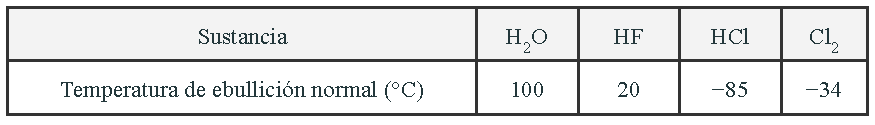
\includegraphics[width=0.65\linewidth]{FigurasSVG/UD3_Enlace_Quimico/pdf/UD3_E02_tabla_ebullicion.pdf}
        \caption{}
        \label{fig:tablaejercicios}
    \end{figure}

    \begin{solu}

%        \begin{figure}[H]
%            \centering
%            \includegraphics[scale=.5]{images/imagesUD3EnlaceQuimico/UD3_Problemas/evauclm12.png}
%        \end{figure}

        \begin{enumerate}[label=\letraminuscula]
            \item El HF es una molécula muy polar en la que el H está unido a un átomo muy electronegativo y pequeño (F), lo que le permite formar \textbf{enlaces de hidrógeno} entre sus moléculas. El HCl, aunque también es polar, no puede formar enlaces de H (el Cl no es lo bastante electronegativo ni pequeño) y solo presenta fuerzas dipolo-dipolo, más débiles. Por eso el punto de ebullición del HF es mayor.

            \item El \ch{H2O} forma \textbf{enlaces de hidrógeno} (además puede formar hasta dos por molécula, ya que tiene dos pares no enlazantes y dos H), mientras que el \ch{Cl2} es una molécula apolar que solo presenta débiles fuerzas de dispersión de London. Por ello, el punto de ebullición del \ch{H2O} es mucho mayor que el del \ch{Cl2}.

            \item Aunque el HCl es una molécula polar (fuerzas dipolo-dipolo) y el \ch{Cl2} es apolar (solo dispersión de London), el \ch{Cl2} tiene muchos más electrones y mayor masa molar que el HCl, lo que genera fuerzas de dispersión más intensas que compensan la ausencia de dipolo permanente. Por eso el punto de ebullición del HCl es menor que el del \ch{Cl2}.

            \item De las cuatro sustancias, el \ch{H2O} presentará el mayor punto de fusión, ya que es la que forma la red de enlaces de hidrógeno más extensa y fuerte (cada molécula puede establecer hasta cuatro enlaces de H con sus vecinas).
        \end{enumerate}
    \end{solu}
\end{exerciseEVAU}

\begin{exerciseEVAU}
    \textbf{2020} Para las siguientes sustancias: \ch{Br2}, \ch{NaCl}, \ch{H2O} y Fe: a) Explicar el tipo de enlace que presentan. b) Indicar el tipo de interacción que debe romperse para fundir cada compuesto.c) ¿Cuál de ellas tendrá un menor punto de fusión? d) Razonar qué compuesto(s) conducirá(n) la corriente en estado sólido, cuál(es) lo hará(n) en estado fundido y cuál(es) no conducirá(n) la corriente eléctrica en ningún caso.


    \begin{solu}

%        \begin{figure}[H]
%            \centering
%            \includegraphics[scale=.5]{images/imagesUD3EnlaceQuimico/UD3_Problemas/evauclm13.png}
%            \includegraphics[scale=.5]{images/imagesUD3EnlaceQuimico/UD3_Problemas/evauclm13b.png}
%        \end{figure}

        \begin{enumerate}[label=\letraminuscula]
            \item \ch{Br2}: molécula \textbf{covalente} apolar. \ch{NaCl}: \textbf{iónico}. \ch{H2O}: molécula \textbf{covalente} polar. Fe: \textbf{metálico}.

            \item Para fundir cada sustancia hay que romper las interacciones \emph{entre} unidades: \ch{Br2} $\to$ fuerzas de dispersión de London; \ch{NaCl} $\to$ atracciones electrostáticas de la red iónica; \ch{H2O} $\to$ enlaces de hidrógeno (y dipolo-dipolo); Fe $\to$ enlace metálico.

            \item El \ch{Br2} tiene el \textbf{menor punto de fusión}, ya que las fuerzas de dispersión de London entre sus moléculas apolares son mucho más débiles que la red iónica del NaCl, los enlaces de H del agua o el enlace metálico del Fe.

            \item El Fe \textbf{conduce en estado sólido} (enlace metálico, electrones deslocalizados libres en todo momento). El NaCl \textbf{no conduce en sólido, pero sí fundido} (o en disolución), ya que solo así los iones quedan libres para desplazarse. El \ch{Br2} y el \ch{H2O} (pura) \textbf{no conducen la corriente en ningún caso}, al ser sustancias covalentes sin iones ni electrones libres.
        \end{enumerate}
    \end{solu}
\end{exerciseEVAU}

\begin{exerciseEVAU}
    \textbf{2020} Explica razonadamente los siguientes hechos: a) El cloruro de sodio tiene un punto de fusión de 801 ºC,
    mientras que el cloro es un gas a temperatura ambiente. b) El metanol es un compuesto muy soluble en agua, mientras que el metano no lo es.
    c) El hierro y el yodo son sólidos a temperatura ambiente; pero el hierro conduce la corriente eléctrica, mientras que el yodo no. d) El cloruro de magnesio es más duro que el cloruro de calcio.

    \begin{solu}

%        \begin{figure}[H]
%            \centering
%            \includegraphics[scale=.5]{images/imagesUD3EnlaceQuimico/UD3_Problemas/evauclm15.png}
%        \end{figure}

        \begin{enumerate}[label=\letraminuscula]
            \item El NaCl es un compuesto \textbf{iónico}, con una red cristalina muy estable mantenida por fuertes fuerzas electrostáticas (alta energía de red), lo que requiere mucha energía para fundirlo. El \ch{Cl2} es una molécula \textbf{covalente apolar} en la que solo actúan débiles fuerzas de dispersión de London entre moléculas, por lo que es gas a temperatura ambiente.

            \item El metanol (\ch{CH3OH}) tiene un grupo --OH capaz de formar \textbf{enlaces de hidrógeno} con el agua, lo que lo hace muy soluble (miscible). El metano (\ch{CH4}) es una molécula apolar, sin capacidad de interaccionar favorablemente con el agua polar, por lo que es prácticamente insoluble.

            \item El Fe tiene \textbf{enlace metálico}: sus electrones de valencia están deslocalizados formando una nube libre de moverse, lo que le confiere conductividad eléctrica. El \ch{I2} es un sólido \textbf{covalente molecular} unido por fuerzas de dispersión de London; sus electrones están localizados en enlaces covalentes y pares solitarios, sin electrones libres, por lo que no conduce la corriente.

            \item El \(\text{Mg}^{2+}\) tiene menor radio iónico que el \(\text{Ca}^{2+}\), por lo que en el \ch{MgCl2} la distancia interiónica es menor y la atracción electrostática (energía de red) es mayor que en el \ch{CaCl2}. Una energía de red mayor implica una red cristalina más fuerte y, por tanto, un compuesto más duro. Por eso el \ch{MgCl2} es más duro que el \ch{CaCl2}.
        \end{enumerate}
    \end{solu}
\end{exerciseEVAU}
\begin{exerciseEVAU}
    \textbf{2021} Sean las moléculas \formula{NH3}, \formula{SO2} y \formula{CO2} a) Deduzca la estructura de Lewis de cada una de ellas. b) Describa la geometría de estas moléculas indicando la hibridación del átomo central. c) Indique el tipo de enlaces $\sigma$/ $\pi$ que se dan en estas moléculas. d) Comente la polaridad de cada molécula.

    \begin{solu}

%        \begin{figure}[H]
%            \centering
%            \includegraphics[scale=.5]{images/imagesUD3EnlaceQuimico/UD3_Problemas/evauclm16a.png}
%            \includegraphics[scale=.5]{images/imagesUD3EnlaceQuimico/UD3_Problemas/evauclm16b.png}
%        \end{figure}

        \begin{enumerate}[label=\letraminuscula]
            \item Las estructuras de Lewis se muestran en la imagen: \ch{NH3} con tres enlaces sencillos N--H y un par no enlazante sobre el N; \ch{SO2} con un doble enlace S=O y un enlace sencillo S--O (estructura resonante) y un par no enlazante sobre el S; \ch{CO2} con dos dobles enlaces \ch{O=C=O}.

            \item \textbf{\ch{NH3}}: tipo \(AB_3E\), geometría \textbf{pirámide trigonal}, hibridación del N: \(\bm{sp^3}\).

            \textbf{\ch{SO2}}: tipo \(AB_2E\), geometría \textbf{angular}, hibridación del S: \(\bm{sp^2}\).

            \textbf{\ch{CO2}}: tipo \(AB_2\), geometría \textbf{lineal}, hibridación del C: \(\bm{sp}\).

            \item \textbf{\ch{NH3}}: 3 enlaces \(\sigma\), sin enlaces \(\pi\). \textbf{\ch{SO2}}: 2 enlaces \(\sigma\) y 1 enlace \(\pi\) deslocalizado entre los dos enlaces S--O. \textbf{\ch{CO2}}: 2 enlaces \(\sigma\) y 2 enlaces \(\pi\).

            \item \textbf{\ch{NH3}}: geometría piramidal asimétrica $\Rightarrow$ \textbf{polar}. \textbf{\ch{SO2}}: geometría angular asimétrica $\Rightarrow$ \textbf{polar}. \textbf{\ch{CO2}}: geometría lineal simétrica, los momentos dipolares se cancelan $\Rightarrow$ \textbf{apolar}.
        \end{enumerate}
    \end{solu}
\end{exerciseEVAU}


\begin{exerciseEVAU}
    \textbf{2021} Justifique, en términos del enlace químico, por qué el \formula{H2O} es un líquido a presión y temperatura ambiente mientras que el \formula{H2S} es un gas en las mismas condiciones. b) Razone que tienen en común los siguientes átomos e iones: \formula{Cl^-}, \formula{Ar} y \formula{K^-}
    \datos{} Z (Cl) =17; Z (Ar) = 18; Z (K) = 19.

    \begin{solu}

%        \begin{figure}[H]
%            \centering
%            \includegraphics[scale=.5]{images/imagesUD3EnlaceQuimico/UD3_Problemas/evauclm17.png}
%        \end{figure}

        El O es mucho más electronegativo y pequeño que el S, lo que permite que las moléculas de \ch{H2O} formen \textbf{enlaces de hidrógeno} entre sí, una interacción intermolecular fuerte que exige mucha energía para separar las moléculas (de ahí que el agua sea líquida a temperatura ambiente). El \ch{H2S}, con un átomo central más grande y menos electronegativo, solo presenta fuerzas dipolo-dipolo y de dispersión, mucho más débiles, por lo que es gaseoso en las mismas condiciones.

        b) (Se entiende el ion del K como \ch{K+}, ya que un anión \ch{K-} no es una especie habitual en química básica). Las especies \ch{Cl-} (\(17+1=18\) electrones), \ch{Ar} (\(18\) electrones) y \ch{K+} (\(19-1=18\) electrones) son \textbf{isoelectrónicas}: todas tienen 18 electrones y la misma configuración electrónica, \( 1s^22s^22p^63s^23p^6 \), la del gas noble Ar.
    \end{solu}
\end{exerciseEVAU}
\begin{exerciseEVAU}
    Considere las moléculas \formula{BF3} y \formula{NH3}. a) Escriba su estructura de Lewis. b) Indique su geometría molecular utilizando la teoría de repulsión de pares de electrones de la capa de valencia. c) Indique cuál es la hibridación del átomo central de cada una de ellas. d) Explique la polaridad de ambas moléculas.

    \begin{solu}
        \begin{enumerate}[label=\letraminuscula]
            \item \textbf{\ch{BF3}}: el B (3 e\textsuperscript{-} de valencia) forma tres enlaces sencillos con los tres F, sin par no enlazante (sexteto sobre el B).

            \textbf{\ch{NH3}}: el N (5 e\textsuperscript{-} de valencia) forma tres enlaces sencillos con los tres H y le queda un par no enlazante.

            \item \textbf{\ch{BF3}}: 3 pares enlazantes, 0 no enlazantes $\Rightarrow$ tipo \(AB_3\), geometría \textbf{trigonal plana}.

            \textbf{\ch{NH3}}: 3 pares enlazantes, 1 no enlazante $\Rightarrow$ tipo \(AB_3E\), geometría \textbf{pirámide trigonal}.

            \item El B en \ch{BF3}, con tres pares de electrones a su alrededor dispuestos en un plano, presenta hibridación \(\bm{sp^2}\).

            El N en \ch{NH3}, con cuatro pares de electrones a su alrededor (3 enlazantes + 1 no enlazante) dispuestos tetraédricamente, presenta hibridación \(\bm{sp^3}\).

            \item \textbf{\ch{BF3}}: los enlaces B--F son polares, pero la simetría trigonal plana hace que los momentos dipolares se cancelen $\Rightarrow$ \textbf{molécula apolar}.

            \textbf{\ch{NH3}}: los enlaces N--H son polares y, debido a la geometría piramidal (asimétrica, con un par no enlazante que refuerza el momento dipolar resultante), los momentos dipolares no se cancelan $\Rightarrow$ \textbf{molécula polar}.
        \end{enumerate}
    \end{solu}
\end{exerciseEVAU}


\begin{exerciseEVAU}
    \textbf{2020} a) La propanona es la cetona más sencilla. a.1) Escribir la fórmula e indicar los enlaces \(\sigma\) y \(\pi\) que forma el átomo de carbono del grupo funcional. a.2) ¿Qué hibridación de los átomos de C puede explicar la estructura de la molécula? a.3) ¿Es una molécula polar? b) Dados los compuestos: ácido 2-hidroxipropanoico, 2-clorobutano y 1-aminoprop-1-eno b.1) Escribir su fórmula semidesarrollada. b.2) ¿Presentan isomería óptica? b.3) ¿Presentan isomería geométrica? Razonar las respuestas.

    \begin{solu}

%        \begin{figure}[H]
%            \centering
%            \includegraphics[scale=.5]{images/imagesUD3EnlaceQuimico/UD3_Problemas/evauclm19.png}
%            \includegraphics[scale=.5]{images/imagesUD3EnlaceQuimico/UD3_Problemas/evauclm19b.png}
%        \end{figure}

        \begin{enumerate}[label=\letraminuscula]
            \item[a.1)] La propanona es \ch{CH3-CO-CH3}. El carbono del grupo carbonilo forma 2 enlaces \(\sigma\) con los dos grupos metilo y, con el oxígeno, un doble enlace C=O formado por 1 enlace \(\sigma\) y 1 enlace \(\pi\).

            \item[a.2)] El carbono carbonílico, rodeado de 3 grupos de electrones (2 enlaces \ch{C-C} y 1 doble enlace C=O), tiene hibridación \(\bm{sp^2}\); los carbonos de los grupos metilo tienen hibridación \(\bm{sp^3}\).

            \item[a.3)] Sí, es una \textbf{molécula polar}: el doble enlace C=O es muy polar (el O es mucho más electronegativo) y la geometría trigonal plana alrededor del carbono carbonílico no permite que ese momento dipolar se cancele con los débiles enlaces C--C.

            \item[b.1)] Ácido 2-hidroxipropanoico (ácido láctico): \ch{CH3-CH(OH)-COOH}. 2-clorobutano: \ch{CH3-CHCl-CH2-CH3}. 1-aminoprop-1-eno: \ch{CH3-CH=CH-NH2}.

            \item[b.2)] El ácido 2-hidroxipropanoico y el 2-clorobutano presentan \textbf{isomería óptica}, ya que ambos tienen un átomo de carbono asimétrico (unido a cuatro sustituyentes distintos): el C2 en cada caso. El 1-aminoprop-1-eno no tiene ningún carbono asimétrico, por lo que \textbf{no presenta isomería óptica}.

            \item[b.3)] Solo el 1-aminoprop-1-eno presenta \textbf{isomería geométrica} (cis-trans), ya que tiene un doble enlace C=C con dos sustituyentes distintos en cada carbono del doble enlace (H/CH3 en un extremo y H/NH2 en el otro), lo que permite las formas cis y trans. Los otros dos compuestos no tienen dobles enlaces C=C y, por tanto, no presentan este tipo de isomería.
        \end{enumerate}
    \end{solu}
\end{exerciseEVAU}
\begin{exerciseEVAU}
    \textbf{ 2020} El propino es un hidrocarburo insaturado. a) Formula el propino y representa el diagrama de Lewis de la molécula. b) ¿Qué hibridación puede explicar los enlaces de los átomos de carbono? c) Escribe la reacción química del propino con bromo en proporción molar 1:1; indica de qué tipo es y nombra el compuesto orgánico formado. d) ¿Cómo afecta la reacción anterior a la hibridación del carbono?

    \begin{solu}

%        \begin{figure}[H]
%            \centering
%            \includegraphics[scale=.5]{images/imagesUD3EnlaceQuimico/UD3_Problemas/evauclm20.png}
%        \end{figure}

        \begin{enumerate}[label=\letraminuscula]
            \item El propino es \ch{HC} \(\equiv\) \ch{C-CH3}. Diagrama de Lewis: triple enlace entre C1 y C2 (cada uno con un par de electrones compartidos triple), C2 unido por enlace sencillo a C3 (\ch{CH3}), y el H terminal unido a C1.

            \item El C1 y el C2 (unidos por el triple enlace) están rodeados de solo 2 grupos de electrones, por lo que tienen hibridación \(\bm{sp}\). El C3 (\ch{CH3}), con cuatro enlaces sencillos, tiene hibridación \(\bm{sp^3}\).

            \item La adición de \ch{Br2} en proporción 1:1 al triple enlace es una \textbf{reacción de adición electrófila}. El \ch{Br2} se adiciona sobre el triple enlace, transformándolo en un doble enlace:
            \begin{center}
                \ch{HC} \(\equiv\) \ch{C-CH3 + Br2 -> CHBr=CBr-CH3}
            \end{center}
            El compuesto orgánico formado es el \textbf{1,2-dibromoprop-1-eno}.

            \item Los dos carbonos que reaccionan (C1 y C2), que partían de hibridación \(sp\) (triple enlace), pasan a tener hibridación \(\bm{sp^2}\) al quedar unidos por un doble enlace tras la adición.
        \end{enumerate}
    \end{solu}
\end{exerciseEVAU}

\begin{exerciseEVAU}
    \textbf{ 2018 } Justifica en términos del enlace químico los siguientes hechos: a) Los metales son dúctiles y maleables, pero los sólidos iónicos no. b) A presión y temperatura ambiente, el cloro (\ch{Cl2}) es un gas, mientras que el bromo (\ch{Br2}) es un líquido.

    \begin{solu}

%        \begin{figure}[H]
%            \centering
%            \includegraphics[scale=.5]{images/imagesUD3EnlaceQuimico/UD3_Problemas/evauclm20nuevo.png}
%        \end{figure}

        \begin{enumerate}[label=\letraminuscula]
            \item En el enlace metálico, los cationes metálicos están rodeados de una nube de electrones deslocalizados que no pertenecen a ningún ion en particular. Al aplicar una fuerza, las capas de cationes pueden deslizarse unas sobre otras sin romper el enlace, ya que la nube electrónica se reajusta y sigue rodeándolos: por eso los metales son dúctiles y maleables. En un sólido iónico, en cambio, cada ion ocupa una posición fija en la red y está unido a sus vecinos de carga opuesta por atracción electrostática; al desplazar una capa, iones de igual carga quedan enfrentados y se repelen fuertemente, lo que fractura el cristal.

            \item Tanto el \ch{Cl2} como el \ch{Br2} son moléculas apolares que solo interaccionan mediante fuerzas de dispersión de London, cuya intensidad aumenta con el tamaño y el número de electrones de la molécula. El \ch{Br2} tiene más electrones y mayor masa molar que el \ch{Cl2}, por lo que sus fuerzas de dispersión son más intensas, dando lugar a un punto de ebullición mayor: por eso el \ch{Br2} es líquido y el \ch{Cl2} gaseoso a temperatura y presión ambiente.
        \end{enumerate}
    \end{solu}
\end{exerciseEVAU}

\begin{exerciseEVAU}
    \textbf{ 2018 } Justifica la certeza o falsedad de las siguientes afirmaciones: a) Los iones \ch{S\mch[2]} y \ch{Ca\pch[2]} son isoelectrónicos. b) Arrancar un electrón a un átomo de K cuesta menos energía que arrancarlo a uno de Cs. c) El átomo de Fe tiene dos electrones desapareados. d) El enlace de la molécula de HF es más polar que el de la molécula de HI.

    \datos{} Números atómicos: F=9; S=16; K=19; Ca=20; Fe=26; I=53; Cs=55.

    \begin{solu}

%        \begin{figure}[H]
%            \centering
%            \includegraphics[scale=.5]{images/imagesUD3EnlaceQuimico/UD3_Problemas/evauclm21.png}
%        \end{figure}

        \begin{enumerate}[label=\letraminuscula]
            \item \textbf{Verdadero}. El \ch{S^{2-}} tiene \(16+2=18\) electrones y el \ch{Ca^{2+}} tiene \(20-2=18\) electrones; ambos comparten la configuración \( 1s^22s^22p^63s^23p^6 \), luego son isoelectrónicos.

            \item \textbf{Falso}. El K (periodo 4) tiene mayor energía de ionización que el Cs (periodo 6), ya que el radio atómico del Cs es mucho mayor (más capas de apantallamiento), lo que hace que su electrón de valencia esté menos atraído por el núcleo. Por tanto, arrancar un electrón cuesta \emph{más} energía en el K que en el Cs.

            \item \textbf{Falso}. La configuración electrónica del Fe es \([\text{Ar}]3d^64s^2\). Según la regla de Hund, los 6 electrones del subnivel \(3d\) (5 orbitales) se distribuyen: los 5 primeros orbitales reciben un electrón cada uno (5 desapareados) y el sexto electrón se aparea en el primer orbital. Por tanto, el Fe tiene \textbf{4 electrones desapareados}, no 2.

            \item \textbf{Verdadero}. La diferencia de electronegatividad entre H y F es mayor que entre H e I (el F es mucho más electronegativo que el I), por lo que el enlace H--F es más polar que el H--I.
        \end{enumerate}
    \end{solu}
\end{exerciseEVAU}
\begin{exerciseEVAU}

    \textbf{ 2018 } Sólo UNA de las siguientes afirmaciones es CORRECTA. Identifícala razonando tu respuesta. a) Los metales son malos conductores de la electricidad. b) Todos los compuestos iónicos son sólidos. c) La unión de un metal con un no metal se produce por enlace covalente. d) Los compuestos iónicos no se disuelven en agua.

    \begin{solu}

%        \begin{figure}[H]
%            \centering
%            \includegraphics[scale=.5]{images/imagesUD3EnlaceQuimico/UD3_Problemas/evauclm22.png}
%        \end{figure}

        La afirmación correcta es la \textbf{b) Todos los compuestos iónicos son sólidos} (a temperatura ambiente, dada su elevada energía de red).

        Las otras son falsas: a) los metales son \emph{buenos} conductores de la electricidad (enlace metálico, electrones deslocalizados); c) la unión de un metal con un no metal da lugar a enlace \textbf{iónico}, no covalente; d) muchos compuestos iónicos, como el NaCl, \textbf{sí se disuelven} en agua.
    \end{solu}
\end{exerciseEVAU}

\begin{exerciseEVAU}
    \textbf{ 2017 } Para los elementos con Z = 9, 12, 16 y 28, a) Indica a qué grupo del sistema periódico pertenece cada uno de ellos. b) ¿Cuál de los cuatro elementos tendrá mayor afinidad electrónica? c) ¿Alguna combinación binaria entre ellos tendrá carácter iónico? d) ¿Cuál o cuáles de los cuatro elementos podrán formar enlace metálico?


    \begin{solu}

%        \begin{figure}[H]
%            \centering
%            \includegraphics[scale=.5]{images/imagesUD3EnlaceQuimico/UD3_Problemas/evauclm23.png}
%        \end{figure}

        \begin{enumerate}[label=\letraminuscula]
            \item \(Z=9\): \(1s^22s^22p^5\), grupo 17 (\textbf{F}, halógenos). \(Z=12\): \(1s^22s^22p^63s^2\), grupo 2 (\textbf{Mg}, alcalinotérreos). \(Z=16\): \(1s^22s^22p^63s^23p^4\), grupo 16 (\textbf{S}, anfígenos). \(Z=28\): \([\text{Ar}]3d^84s^2\), grupo 10 (\textbf{Ni}, metales de transición).

            \item El \(F\) (\(Z=9\)) tendrá la \textbf{mayor afinidad electrónica}, ya que los halógenos, pequeños y muy electronegativos, son los elementos con mayor tendencia a captar un electrón.

            \item Sí: por ejemplo, la combinación entre Mg (metal) y F o S (no metales) presenta gran diferencia de electronegatividad, dando lugar a compuestos de carácter \textbf{iónico} (\ch{MgF2} o \ch{MgS}).

            \item El Mg y el Ni son los dos elementos metálicos, por lo que ambos pueden formar enlace metálico.
        \end{enumerate}
    \end{solu}
\end{exerciseEVAU}

\begin{exerciseEVAU}
    \textbf{ 2017 } Formula el compuesto 2-propenol (propen-2-ol, 1-propen-2-ol) y responde a las siguientes cuestiones: a) ¿Cuál es la hibridación de los átomos de carbono 2 y 3? b) De todos los enlaces de esta molécula, cuál es el enlace más polar? Indica, además, un enlace sigma (\(\sigma\)) y un enlace pi (\(\pi\)). c) Formula y nombra un isómero de función del 2-propenol.

    \begin{solu}

%        \begin{figure}[H]
%            \centering
%            \includegraphics[scale=.5]{images/imagesUD3EnlaceQuimico/UD3_Problemas/evauclm24.png}
%        \end{figure}

        El 2-propenol es \ch{CH2=C(OH)-CH3} (\(\text{C1}{=}\text{CH}_2\), \(\text{C2}{=}\text{C(OH)}\), \(\text{C3}{=}\text{CH}_3\)).

        \begin{enumerate}[label=\letraminuscula]
            \item El C2, que forma parte del doble enlace \ch{C1=C2} y está además unido al --OH, está rodeado de 3 grupos de electrones, por lo que tiene hibridación \(\bm{sp^2}\). El C3 (\ch{CH3}), con cuatro enlaces sencillos, tiene hibridación \(\bm{sp^3}\).

            \item El enlace más polar de la molécula es el \textbf{O--H} (mayor diferencia de electronegatividad entre O y H que entre C y O). Un ejemplo de enlace \(\sigma\) es el enlace \ch{C2-C3}; un ejemplo de enlace \(\pi\) es el que forma parte del doble enlace \ch{C1=C2}.

            \item Un isómero de función del 2-propenol (fórmula \ch{C3H6O}) es la \textbf{propanona (acetona)}, \ch{CH3-CO-CH3} (o también el propanal, \ch{CH3-CH2-CHO}): mismo número y tipo de átomos, pero con función cetona (o aldehído) en lugar de enol.
        \end{enumerate}
    \end{solu}
\end{exerciseEVAU}

\begin{exerciseEVAU}
    \textbf{2017}. Sólo UNA de las siguientes afirmaciones es FALSA. Identifícala razonando todas tus respuestas. a) El cloruro de potasio (KCl) conduce la electricidad en estado fundido. b) A temperatura ambiente, todas las sustancias covalentes son gases. c) El diamante, siendo una sustancia covalente, tiene un punto de fusión muy alto. d) Todos los metales son buenos conductores de la electricidad.
    \begin{solu}
%        \begin{figure}[H]
%            \centering
%            \includegraphics[scale=.5]{images/imagesUD3EnlaceQuimico/UD3_Problemas/evauclm25.png}
%        \end{figure}

        La afirmación \textbf{falsa} es la \textbf{b) A temperatura ambiente, todas las sustancias covalentes son gases}: existen sustancias covalentes moleculares sólidas (como el diamante o el propio azúcar) y líquidas (como el agua), no solo gaseosas.

        Las otras son verdaderas: a) el KCl, compuesto iónico, conduce fundido (los iones quedan libres para moverse); c) el diamante, sólido covalente atómico con una red tridimensional de enlaces C--C muy fuertes, tiene un punto de fusión muy elevado; d) todos los metales, gracias al enlace metálico, son buenos conductores de la electricidad.
    \end{solu}
\end{exerciseEVAU}

% \newpage

% \begin{table}[H]
%     \centering
%     \begin{tblr}{|Q[c,m]|Q[c,m]|}
%         \hline
%         {\textbf{Geometría}                                                                                                   \\ (cuando los átomos unidos al átomo central son iguales)} & \textbf{Polaridad}\\
%         \hline
%         {\includegraphics[scale=.5]{images/imagesUD3EnlaceQuimico/UD3_Problemas/lineal.png}  Lineal}                                                  & Apolar \\
%         \hline
%         {\includegraphics[scale=0.5]{images/imagesUD3EnlaceQuimico/UD3_Problemas/trigonal.png}  Trigonal plana (triangular)}                          & Polar  \\
%         \hline
%         {\includegraphics[scale=0.5]{images/imagesUD3EnlaceQuimico/UD3_Problemas/angular.png} Angular}                                                & Polar  \\
%         \hline
%         {\includegraphics[scale=0.5]{images/imagesUD3EnlaceQuimico/UD3_Problemas/tetraedrica.png} Tetraédrica }                                       & Apolar \\
%         \hline
%         {\includegraphics[scale=.5]{images/imagesUD3EnlaceQuimico/UD3_Problemas/piramidetrigonal.png}  Pirámide trigonal}                             & Polar  \\
%         \hline
%         {\includegraphics[scale=.5]{images/imagesUD3EnlaceQuimico/UD3_Problemas/bipiramidetrigonal.png}  Bipirámide trigonal (bipirámide triangular)} & Polar  \\
%         \hline
%         {\includegraphics[scale=.5]{images/imagesUD3EnlaceQuimico/UD3_Problemas/tetraedricadistorsionada.png} Tetraédrica distorsionada }             & Polar  \\
%         \hline
%         {\includegraphics[scale=.5]{images/imagesUD3EnlaceQuimico/UD3_Problemas/enformadeT.png} En forma de T}                                        & Polar  \\
%         \hline
%         {\includegraphics[scale=.5]{images/imagesUD3EnlaceQuimico/UD3_Problemas/octaedrica.png}  Octaédrica}                                          & Apolar \\
%         \hline
%         {\includegraphics[scale=.5]{images/imagesUD3EnlaceQuimico/UD3_Problemas/piramidalcuadrada.png}  Pirámide cuadrada}                            & Polar  \\
%         \hline
%         {\includegraphics[scale=.5]{images/imagesUD3EnlaceQuimico/UD3_Problemas/planacuadrada.png}  Plano cuadrada}                                   & Apolar \\
%         \hline
%     \end{tblr}
% \end{table}

% \begin{table}[H]
%     \centering
%     \begin{tblr}{|Q[c,m]|Q[c,m]|Q[c,m]|Q[c,m]|Q[c,m]|}
%         \hline
%         {\textbf{nº total de}                                                                                                                                                           \\ \textbf{pares de \el}} & {\textbf{nº total de pares} \\ \textbf{de \el enlazantes}} & {\textbf{nº total de pares} \\ \textbf{de \el no enlazantes}} &\textbf{Geometría} & \textbf{Ejemplo}\\
%         \hline
%         2                  & 2 & 0 & {\includegraphics[scale=.5]{images/imagesUD3EnlaceQuimico/UD3_Problemas/lineal.png}                                                      Lineal}                       & \ch{BeF2}  \\
%         \hline
%         \SetCell[r=2]{m} 3 & 3 & 0 & {\includegraphics[scale=.5]{images/imagesUD3EnlaceQuimico/UD3_Problemas/trigonal.png}                                                     Trigonal plana (triangular)} & \ch{BeF2}  \\
%         \hline
%                            & 2 & 1 & {\includegraphics[scale=.5]{images/imagesUD3EnlaceQuimico/UD3_Problemas/angular.png} Angular   }                                                                       & \ch{SnCl2} \\
%         \hline
%         \SetCell[r=3]{m} 4 & 4 & 0 & {\includegraphics[scale=.5]{images/imagesUD3EnlaceQuimico/UD3_Problemas/tetraedrica.png} Tetraédrica }                                                                 & \ch{CH4}   \\
%         \hline
%                            & 3 & 1 & {\includegraphics[scale=.5]{images/imagesUD3EnlaceQuimico/UD3_Problemas/piramidetrigonal.png} Pirámide trigonal }                                                      & \ch{NH3}   \\
%         \hline
%                            & 2 & 2 & {\includegraphics[scale=.5]{images/imagesUD3EnlaceQuimico/UD3_Problemas/angularb.png} Angular }                                                                        & \ch{H2O}   \\
%         \hline
%         \SetCell[r=4]{m} 5 & 5 & 0 & {\includegraphics[scale=.5]{images/imagesUD3EnlaceQuimico/UD3_Problemas/bipiramidetrigonal.png} Bipirámide triangular}                                                 & \ch{PCl5}  \\
%         \hline
%                            & 4 & 1 & {\includegraphics[scale=.5]{images/imagesUD3EnlaceQuimico/UD3_Problemas/tetraedricadistorsionada.png} Tetraédrica distorsionada}                                       & \ch{SF4}   \\
%         \hline
%                            & 3 & 2 & {\includegraphics[scale=.5]{images/imagesUD3EnlaceQuimico/UD3_Problemas/enformadeT.png} En forma de T  }                                                               & \ch{ClF3}  \\
%         \hline
%                            & 2 & 3 & {\includegraphics[scale=.5]{images/imagesUD3EnlaceQuimico/UD3_Problemas/linealb.png} Lineal  }                                                                         & \ch{XeF2}  \\
%         \hline
%         \SetCell[r=3]{m}6  & 6 & 0 & {\includegraphics[scale=.5]{images/imagesUD3EnlaceQuimico/UD3_Problemas/octaedrica.png} Octaédrica}                                                                    & \ch{SF6}   \\
%         \hline
%                            & 5 & 1 & {\includegraphics[scale=.5]{images/imagesUD3EnlaceQuimico/UD3_Problemas/piramidalcuadrada.png} Pirámide cuadrada}                                                      & \ch{ICl5}  \\
%         \hline
%                            & 4 & 2 & {\includegraphics[scale=.5]{images/imagesUD3EnlaceQuimico/UD3_Problemas/planacuadrada.png} Plano cuadrada}                                                             & \ch{XeF4}  \\
%         \hline
%     \end{tblr}
% \end{table}

